%% abtex2-modelo-trabalho-academico.tex, v-1.9.3 laurocesar
%% Copyright 2012-2015 by abnTeX2 group at http://abntex2.googlecode.com/ 
%% This work may be distributed and/or modified under the
%% conditions of the LaTeX Project Public License, either version 1.3
%% of this license or (at your option) any later version.
%% The latest version of this license is
%%   http://www.latex-project.org/lppl.txt
%% and version 1.3 or later is part of all distributions of LaTeX
%% version 2005/12/01 or later.
%%
%% This work has the LPPL maintenance status `maintained'.
%% 
%% The Current Maintainer of this work is the abnTeX2 team, led
%% by Lauro César Araujo. Further information are available on 
%% http://abntex2.googlecode.com/
%%
%% This work consists of the files abntex2-modelo-trabalho-academico.tex,
%% abntex2-modelo-include-comandos and abntex2-modelo-references.bib
%%

% ------------------------------------------------------------------------
% ------------------------------------------------------------------------
% abnTeX2: Modelo de Trabalho Academico (tese de doutorado, dissertacao de
% mestrado e trabalhos monograficos em geral) em conformidade com 
% ABNT NBR 14724:2011: Informacao e documentacao - Trabalhos academicos -
% Apresentacao
% ------------------------------------------------------------------------
% ------------------------------------------------------------------------

\documentclass[
	% -- opções da classe memoir --
	12pt,				% tamanho da fonte
	openright,			% capítulos começam em pág ímpar (insere página vazia caso preciso)
	% twoside,			% para impressão em verso e anverso. Oposto a oneside
	oneside,			% mantém margens uniformes em todas as páginas
	a4paper,			% tamanho do papel. 
	% -- opções da classe abntex2 --
	%chapter=TITLE,		% títulos de capítulos convertidos em letras maiúsculas
	%section=TITLE,		% títulos de seções convertidos em letras maiúsculas
	%subsection=TITLE,	% títulos de subseções convertidos em letras maiúsculas
	%subsubsection=TITLE,% títulos de subsubseções convertidos em letras maiúsculas
	% -- opções do pacote babel --
	english,			% idioma adicional para hifenização
	brazilian			% o último idioma é o principal do documento
	]{abntex2}

% ---
% Pacotes básicos 
% ---
%\usepackage{uarial}				% Usa a fonte Latin Modern			lmodern
\usepackage[T1]{fontenc}		% Selecao de codigos de fonte.
\usepackage[utf8]{inputenc}		% Codificacao do documento (conversão automática dos acentos)
\usepackage{lmodern}
\usepackage{footnote}
\usepackage{lastpage}			% Usado pela Ficha catalográfica
\usepackage{indentfirst}		% Indenta o primeiro parágrafo de cada seção.
\usepackage{color}				% Controle das cores
\usepackage{graphicx}			% Inclusão de gráficos
\usepackage{microtype} 			% para melhorias de justificação

% pacotes adicionados
\usepackage{amsmath}
\usepackage{float}
\usepackage{amssymb,amsfonts,amsthm}
\usepackage{setspace}
\usepackage{listings}
\usepackage{hyperref}
\usepackage{caption}
% ---
		
% ---
% Pacotes adicionais, usados apenas no âmbito do Modelo Canônico do abnteX2
% ---
\usepackage{lipsum}				% para geração de dummy text
% ---
% ---
% Pacotes de citações
% ---
\usepackage[brazilian,hyperpageref]{backref}	 % Paginas com as citações na bibl
\usepackage[alf]{abntex2cite}	% Citações padrão ABNT
\renewcommand{\bf}[1]{\mathbf{#1}}
\renewcommand{\rm}[1]{\mathrm{#1}}

% \usepackage{cite}
%\renewcommand\citeleft{[}
%\renewcommand\citeright{]}

% Altera o nome padrão do rótulo usado no comando \autoref{}
\renewcommand{\lstlistingname}{Código}

% Altera o rótulo a ser usando no elemento pré-textual "Lista de código"
\renewcommand{\lstlistlistingname}{Lista de códigos}

% Configura a ``Lista de Códigos'' conforme as regras da ABNT (para abnTeX2)
\begingroup\makeatletter
\let\newcounter\@gobble\let\setcounter\@gobbletwo
  \globaldefs\@ne \let\c@loldepth\@ne
  \newlistof{listings}{lol}{\lstlistlistingname}
  \newlistentry{lstlisting}{lol}{0}
\endgroup

\renewcommand{\cftlstlistingaftersnum}{\hfill--\hfill}

\let\oldlstlistoflistings\lstlistoflistings
\renewcommand{\lstlistoflistings}{%
   \begingroup%
   \let\oldnumberline\numberline%
   \renewcommand{\numberline}{\lstlistingname\space\oldnumberline}%
   \oldlstlistoflistings%
   \endgroup}

% Cria uma nova customização para a linguagem Python
\lstloadlanguages{Python}
\lstdefinestyle{pythonCustom}{
  alsoother={0123456789_},
  backgroundcolor=\color{white},   % choose the background color; you must add \usepackage{color} or \usepackage{xcolor}
  % the size of the fonts that are used for the code
  basicstyle=\ttfamily\ABNTEXfontereduzida, 
  % backgroundcolor=\color{theshade},
  breakatwhitespace=false,         % sets if automatic breaks should only happen at whitespace
  breaklines=true,                 % sets automatic line breaking
  captionpos=b,                    % sets the caption-position to bottom
  commentstyle=\color{olive},    % comment style
  deletekeywords={...},            % if you want to delete keywords from the given language
  escapeinside={\%*}{*)},          % if you want to add LaTeX within your code
  extendedchars=true,              % lets you use non-ASCII characters; for 8-bits encodings only, does not work with UTF-8
  frame=single,                    % adds a frame around the code
  inputencoding=utf8,
  keepspaces=true,                 % keeps spaces in text, useful for keeping indentation of code (possibly needs columns=flexible)
  keywordstyle=\color{blue},       % keyword style
  language=Python,                 % the language of the code
  literate={á}{{\'a}}1 {ã}{{\~a}}1 {é}{{\'e}}1 {è}{{\`{e}}}1 {ê}{{\^{e}}}1 {ë}{{\¨{e}}}1 {É}{{\'{E}}}1 {Ê}{{\^{E}}}1 {û}{{\^{u}}}1 {ú}{{\'{u}}}1 {â}{{\^{a}}}1 {à}{{\`{a}}}1 {á}{{\'{a}}}1 {ã}{{\~{a}}}1 {Á}{{\'{A}}}1 {Â}{{\^{A}}}1 {Ã}{{\~{A}}}1 {ç}{{\c{c}}}1 {Ç}{{\c{C}}}1 {õ}{{\~{o}}}1 {ó}{{\'{o}}}1 {ô}{{\^{o}}}1 {Õ}{{\~{O}}}1 {Ó}{{\'{O}}}1 {Ô}{{\^{O}}}1 {î}{{\^{i}}}1 {Î}{{\^{I}}}1 {í}{{\'{i}}}1 {Í}{{\~{Í}}}1,
  % if you want to add more keywords to the set
  morekeywords={*, :-},
  numberbychapter=false,
  numbers=left,                    % where to put the line-numbers; possible values are (none, left, right)
  numbersep=5pt,                   % how far the line-numbers are from the code
  % the style that is used for the line-numbers
  numberstyle=\tiny\color{gray}\sffamily, 
  rulecolor=\color{gray},         % if not set, the frame-color may be changed on line-breaks within not-black text (e.g. comments (green here))
  showspaces=false,                % show spaces everywhere adding particular underscores; it overrides 'showstringspaces'
  showstringspaces=false,          % underline spaces within strings only
  showtabs=false,                  % show tabs within strings adding particular underscores
  stepnumber=1,                    % the step between two line-numbers. If it's 1, each line will be numbered
  stringstyle=\color{olive}\itshape,     % string literal style
  tabsize=1,                       % sets default tabsize to 2 spaces
  title=\lstname,                  % show the filename of files included with \lstinputlisting; also try caption instead of title
  framexleftmargin=10pt,
  framexleftmargin=15pt
}
\lstset{escapechar=@,style=pythonCustom}

% --- 
% CONFIGURAÇÕES DE PACOTES
% --- 
\renewcommand{\imprimircapa}{
\thispagestyle{empty}

\vfill
 \begin{center}
    

    {\large\bfseries UNIVERSIDADE VILA VELHA} \\
    

    \vspace*{1in}
    \begin{large} \bfseries LUCAS MORAIS GOMES \\ NATHALIA DIAS FELIPE \end{large}\\[0.4in]

    \vspace*{4cm}
    {\Large \textsc\textbf{{A TECNOLOGIA COMO FERRAMENTA DE APOIO AO CONTROLE FINANCEIRO} }}\\
    \vspace{1cm}
    \noindent \\
    
    \large\bfseries{}
    \vfill
    \large\bfseries{VILA VELHA \\2026}
\end{center}

\normalsize


}


\renewcommand{\imprimirfolhaderosto}{

\begin{center}

    {\large LUCAS MORAIS GOMES \\ NATHALIA DIAS FELIPE\\}
    \vspace{8cm}
    {\Large \textsc\textbf{{A TECNOLOGIA COMO FERRAMENTA DE APOIO AO CONTROLE FINANCEIRO} }\\}
    \vspace{1cm}
    \hspace{.45\linewidth}
    \begin{minipage}{.50\linewidth}

            \textbf{Trabalho de conclusão de curso apresentado a Universidade Vila Velha, como requisito parcial para obtenção do grau de Bacharel em Sistemas de Informação. Orientador: Prof. Gabriela de Jesus Martins. }

           
    
    \end{minipage}

    \vspace{2cm}
    \vfill
    {\large Vila Velha, \today{}}
\end{center}

}


% ---
% Configurações do pacote backref
% Usado sem a opção hyperpageref de backref
\renewcommand{\backrefpagesname}{Citado na(s) página(s):~}
% Texto padrão antes do número das páginas
\renewcommand{\backref}{}
% Define os textos da citação
\renewcommand*{\backrefalt}[4]{
	\ifcase #1 %
		Nenhuma citação no texto.%
	\or
		Citado na página #2.%
	\else
		Citado #1 vezes nas páginas #2.%
	\fi}%
% ---
% Configurações de aparência do PDF final

% alterando o aspecto da cor azul
\definecolor{blue}{RGB}{41,5,195}

% informações do PDF
\makeatletter
\hypersetup{
     	%pagebackref=true,
		colorlinks=true,       		% false: boxed links; true: colored links
    	linkcolor=blue,          	% color of internal links
    	citecolor=black,        		% color of links to bibliography
    	filecolor=magenta,      		% color of file links
		urlcolor=blue,
		bookmarksdepth=4
}



\makeatother
% --- 

% --- 
% Espaçamentos entre linhas e parágrafos 
% --- 

% O tamanho do parágrafo é dado por:
\setlength{\parindent}{1.3cm}

% Controle do espaçamento entre um parágrafo e outro:
\setlength{\parskip}{0.2cm}  % tente também \onelineskip

% ---
% compila o indice
% ---
\makeindex
% ---

% ----
% Início do documento
% ----
\begin{document}

% Seleciona o idioma do documento (conforme pacotes do babel)
%\selectlanguage{english}
\selectlanguage{brazilian}

% Retira espaço extra obsoleto entre as frases.
\frenchspacing 

% ----------------------------------------------------------
% ELEMENTOS PRÉ-TEXTUAIS
% ----------------------------------------------------------
\pretextual

% ---
% Capa
% ---
\imprimircapa
% ---

% ---
% Folha de rosto
% (o * indica que haverá a ficha bibliográfica)
% ---
\imprimirfolhaderosto

\include{ficha}
%\include{errata}
% ---
% Inserir folha de aprovação
% ---

% Isto é um exemplo de Folha de aprovação, elemento obrigatório da NBR
% 14724/2011 (seção 4.2.1.3). Você pode utilizar este modelo até a aprovação
% do trabalho. Após isso, substitua todo o conteúdo deste arquivo por uma
% imagem da página assinada pela banca com o comando abaixo:
%
% \includepdf{folhadeaprovacao_final.pdf}
%
\begin{folhadeaprovacao}


\begin{center}


            {UNIVERSIDADE VILA VELHA} \\
           

    \vspace{1.5cm}
                                    {LUCAS MORAIS GOMES \\ NATHALIA DIAS FELIPE}\\
    \bfseries{}
\end{center}

Esta Monografia foi julgada adequada para a obten\c{c}\~{a}o do título  de Bacharel em Sistemas de Informação, sendo aprovada em sua forma final  pela banca examinadora:

    \vspace{2.5cm}
    \assinatura{Orientador: Prof. Gabriela Martins \\ Universidade Vila Velha - UVV}
    \assinatura{Avaliador: Prof. Zezinho \\ Universidade Vila Velha - UVV}
    %\vspace{3 cm}
    \vfill

    \begin{center}
        Vila Velha, \today{}
    \end{center}
  
\end{folhadeaprovacao}
%\include{dedicatoria}
%\include{agradecimentos}
% \include{epigrafe}
% ---
% RESUMOS
% ---

% resumo em portugues
\setlength{\absparsep}{18pt}
\begin{resumo}
Este trabalho propõe o desenvolvimento de um chatbot financeiro integrado ao WhatsApp para auxiliar usuários no registro e acompanhamento de entradas, saídas e metas financeiras por meio de linguagem natural. A proposta combina automação de mensagens, classificação de despesas, geração de relatórios e visualização de dados em interface web, buscando reduzir o esforço de registro manual e aumentar a constância no controle financeiro pessoal. A pesquisa adota abordagem qualitativa e exploratória, com levantamento de dados junto a usuários para identificar hábitos, dificuldades e expectativas relacionadas à organização financeira. A partir desses insumos, são definidos requisitos, artefatos de modelagem e diretrizes para a solução técnica. Espera-se que o sistema contribua para um processo de controle financeiro mais acessível, prático e aderente ao cotidiano dos usuários.

\textbf{Palavras-chave}: Chatbot financeiro, WhatsApp, Controle financeiro, Linguagem natural, Automação, Inteligência Artificial.
\end{resumo}

% resumo em ingles
\begin{resumo}[Abstract]
\begin{otherlanguage*}{english}
This work proposes the development of a financial chatbot integrated with WhatsApp to help users record and monitor income, expenses, and financial goals through natural language. The solution combines message automation, expense classification, report generation, and data visualization in a web interface, aiming to reduce the effort required for manual record keeping and to improve consistency in personal financial management. The research adopts a qualitative and exploratory approach, using user data collection to identify habits, difficulties, and expectations related to financial organization. Based on these findings, requirements, modeling artifacts, and guidelines for the technical solution are defined. The expected outcome is a system that supports a more accessible, practical, and everyday-oriented financial control process.

\textbf{Keywords}: Financial chatbot, WhatsApp, Financial management, Natural language, Automation, Artificial Intelligence.
\end{otherlanguage*}
\end{resumo}
% ---

% ---
% inserir lista de ilustrações
% ---
\pdfbookmark[0]{\listfigurename}{lof}
\listoffigures*
\cleardoublepage
% ---
% inserir lista de tabelas
% ---
\pdfbookmark[0]{\listtablename}{lot}
\listoftables*
\cleardoublepage


% ---
% inserir lista de listings
% ---
%\pdfbookmark[0]{\lstlistlistingname}{lol}
%\begin{KeepFromToc}
%{   % Straightforward hack to remove footnote marks from lstlistoflistings
%\let\footnotemark\relax
%\lstlistoflistings
%}
%\end{KeepFromToc}
%\cleardoublepage

% ---
% ---
% inserir lista de abreviaturas e siglas
% ---
\begin{siglas}
 \item PLN Processamento de Linguagem Natural
\end{siglas}
% ---

% ---
% inserir lista de símbolos
% ---
%\begin{simbolos}
%  \item[$ CO_2 $] Dióxido de Carbono
%  \item[$C_{3+}$] Hidrocarbonetos com três ou mais carbonos
%\end{simbolos}
% ---





% ---
% inserir o sumario
%% ---
\pdfbookmark[0]{\contentsname}{toc}
\tableofcontents*
\cleardoublepage
%% ---



% ----------------------------------------------------------
% ELEMENTOS TEXTUAIS
% ----------------------------------------------------------
\textual

\chapter{Introdução}

Para compreender plenamente o papel dos jogos na sociedade, inclusive no contexto contemporâneo, é necessário visualizar sua trajetória histórica. O primeiro jogo de que se tem registro é o Senet, originário do Antigo Egito por volta de 3100 a.C.

Tratava-se de um jogo de tabuleiro praticado por faraós, que carregava significados espirituais profundos, simbolizando, segundo os estudiosos, a jornada da alma no pós-vida. Vestígios de tabuleiros de Senet foram encontrados em diversas tumbas egípcias, inclusive na do faraó Tutancâmon conforme a imagem \citeonline{piccione1980}.

Desde então, os jogos têm acompanhado o desenvolvimento da humanidade, refletindo aspectos culturais, religiosos e sociais.

\begin{figure}[H]
    \centering
    
    \label{fig:Senet}
    \caption{Pintura mural em uma tumba na necrópole de Tebas, no Egito Antigo}
    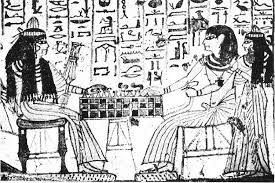
\includegraphics[width=0.8\textwidth]{figs/Senet.jpeg} 
    
    Fonte: {\cite{piccione1980}}.
\end{figure}

Com o avanço da tecnologia e o maior acesso aos meios digitais, a indústria de jogos vem se fortalecendo e crescendo a cada dia. Em 2020, a quantidade de pessoas que jogam regularmente algum tipo de jogo chegou a 3,1 bilhões, representando 40\% da população mundial\footnote{\url{https://www.dfcint.com/dossier/global-video-game-consumer-population/}, acessado em \today.}, sendo utilizada como forma de entretenimento, distração, passatempo e até mesmo como fonte de renda para algumas pessoas. Essa grande popularidade talvez se deva à diversidade de interesses e aos diferentes níveis de complexidade que os jogos oferecem.

Um exemplo disso são os jogos de palavras, um nicho tão antigo quanto os jornais. Tais jogos vêm ganhando destaque nos meios digitais, como é o caso do \textit{Wordle}, que desafia o participante a descobrir uma palavra de cinco letras por meio de feedbacks interativos, o qual evidenciou ainda mais o grande interesse do público por quebra-cabeças linguísticos, sendo inclusive adquirido pelo maior jornal do mundo, o \textit{The New York Times}\footnote{\url{https://www.nytimes.com/2022/01/31/business/media/new-york-times-wordle.html}, acessado em \today.}.

\begin{figure}[H]
    \centering
    
    \label{fig:wordle}
    \caption{Interface do jogo Wordle sendo utilizada em um smartphone}
    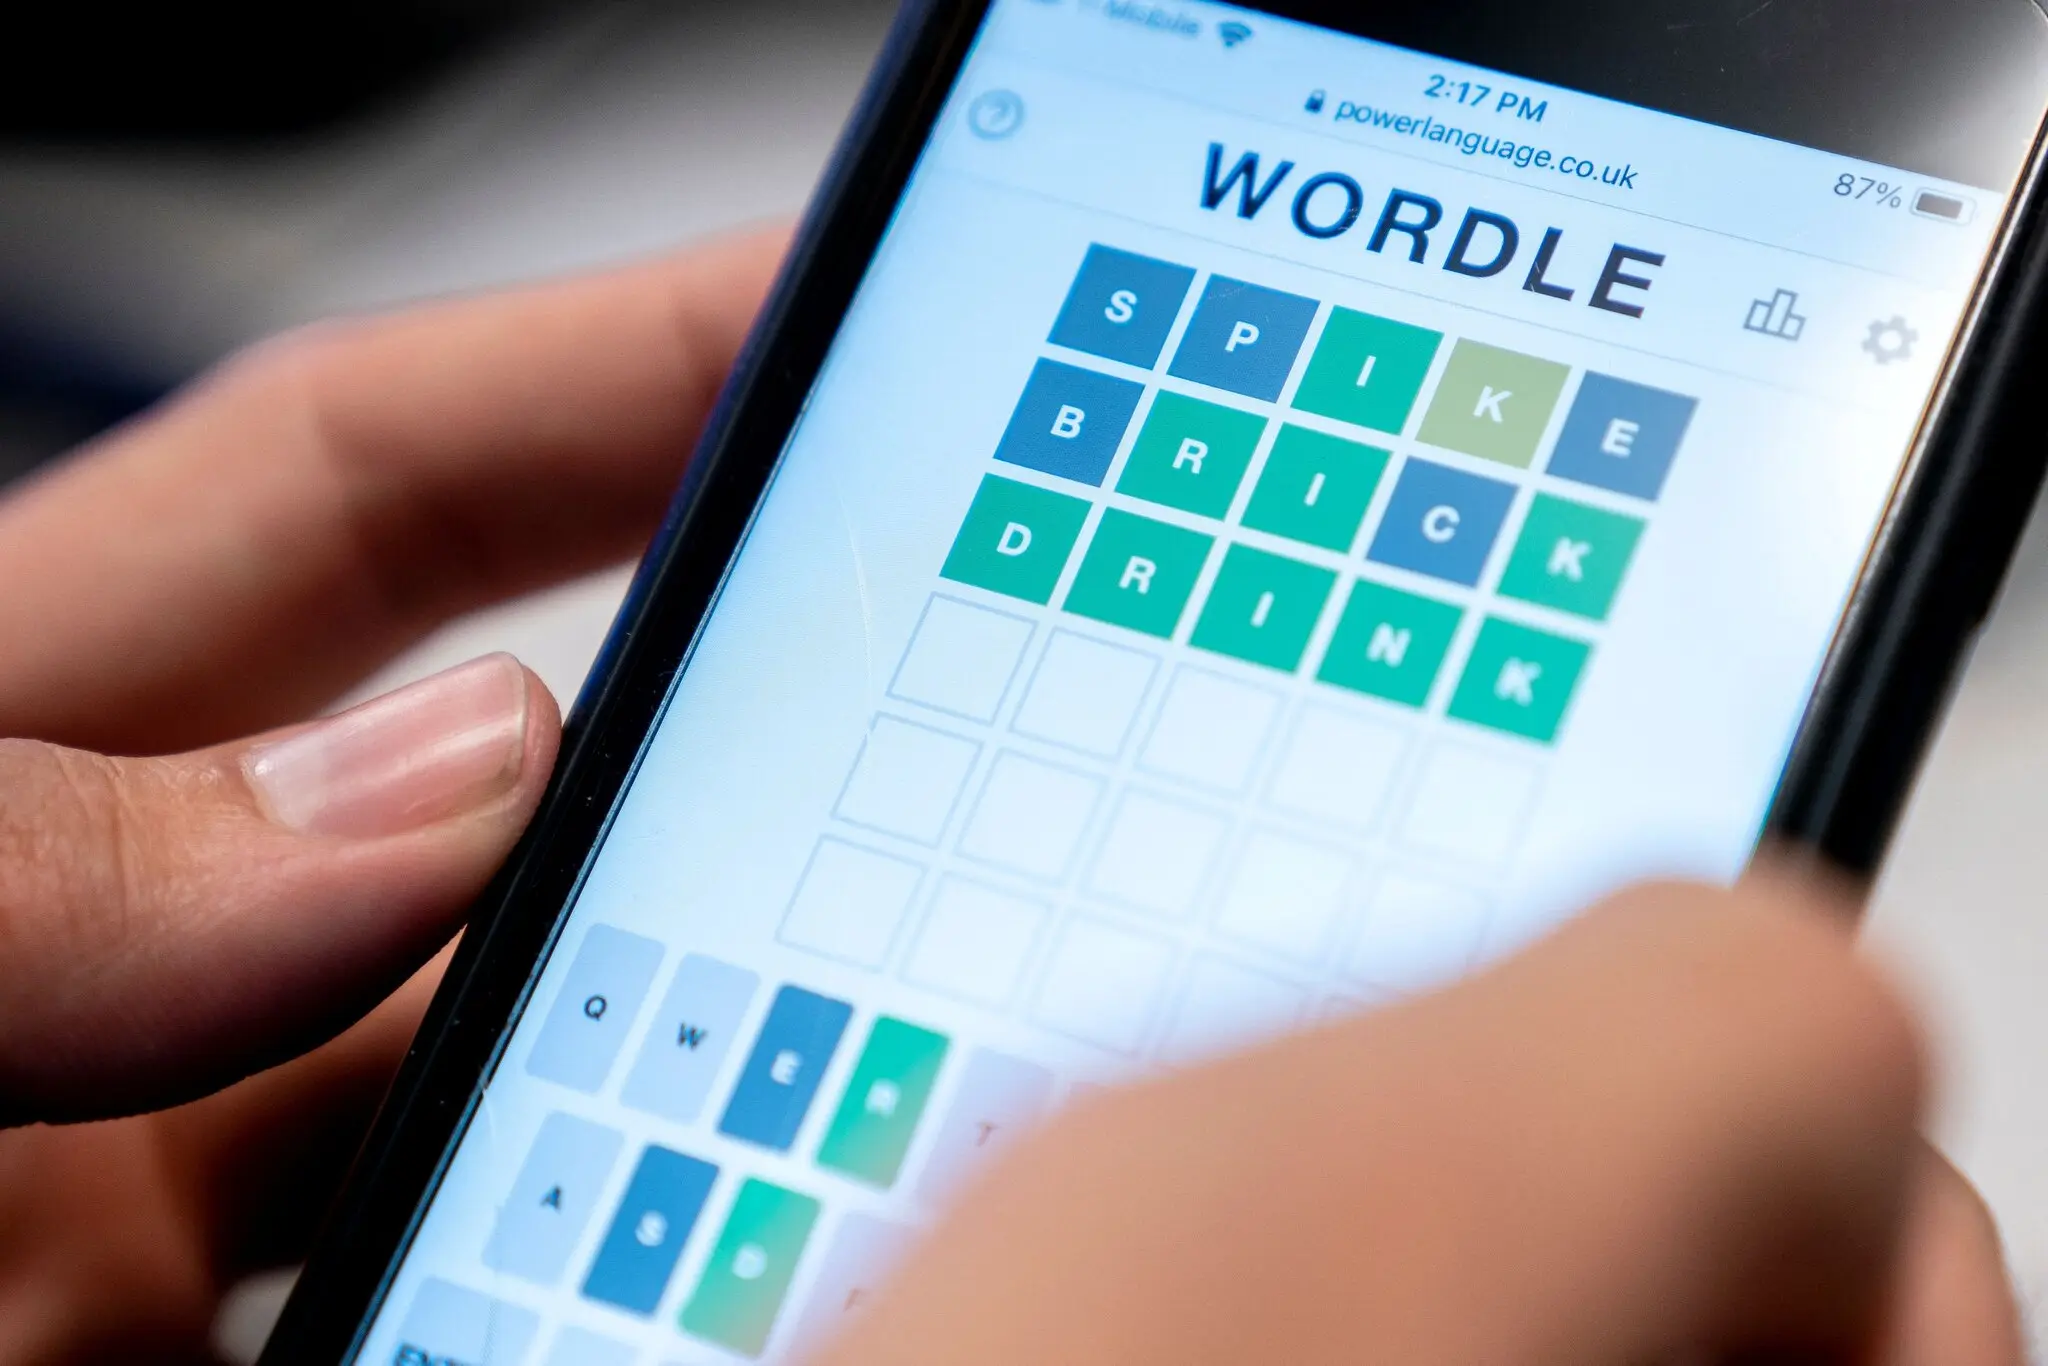
\includegraphics[width=0.8\textwidth]{figs/wordle.png} 
    
   Fonte: \cite{nyt2022wordle}
\end{figure}

Além disso, não é de hoje que grandes jogos passam por transformações significativas com o avanço da tecnologia. O xadrez, jogo de origem milenar e altamente estratégico, tornou-se um marco no campo da Inteligência Artificial (IA), uma vez que foi o primeiro a ser amplamente estudado e "automatizado" em ambientes virtuais. Isso se deu por sua complexidade lógica e previsibilidade de regras, motivo pelo qual foi considerado, durante décadas, o grande desafio da IA.

Nesse contexto, a vitória do computador \textit{Deep Blue}, desenvolvido pela \textit{International Business Machines} (IBM), sobre o campeão mundial Garry Kasparov em 1997 simbolizou um divisor de águas, ao demonstrar a capacidade das máquinas em superar habilidades humanas em tarefas cognitivas complexas \cite{campbell200257}. No entanto, isso não representou algo negativo. Anos após a derrota, o próprio Kasparov afirmou, em uma de suas palestras, que “devemos enfrentar nossos temores se quisermos tirar o máximo proveito da tecnologia... e devemos derrotar esses temores se quisermos tirar o máximo proveito da humanidade” \cite{kasparov2017}, reconhecendo a utilidade da inteligência artificial como ferramenta e destacando que devemos extrair ao máximo suas vantagens.

\begin{figure}[H]
    \centering
    
    \label{fig:kasparovXdeepBlue}
    \caption{Garry Kasparov contra Deep Blue}
    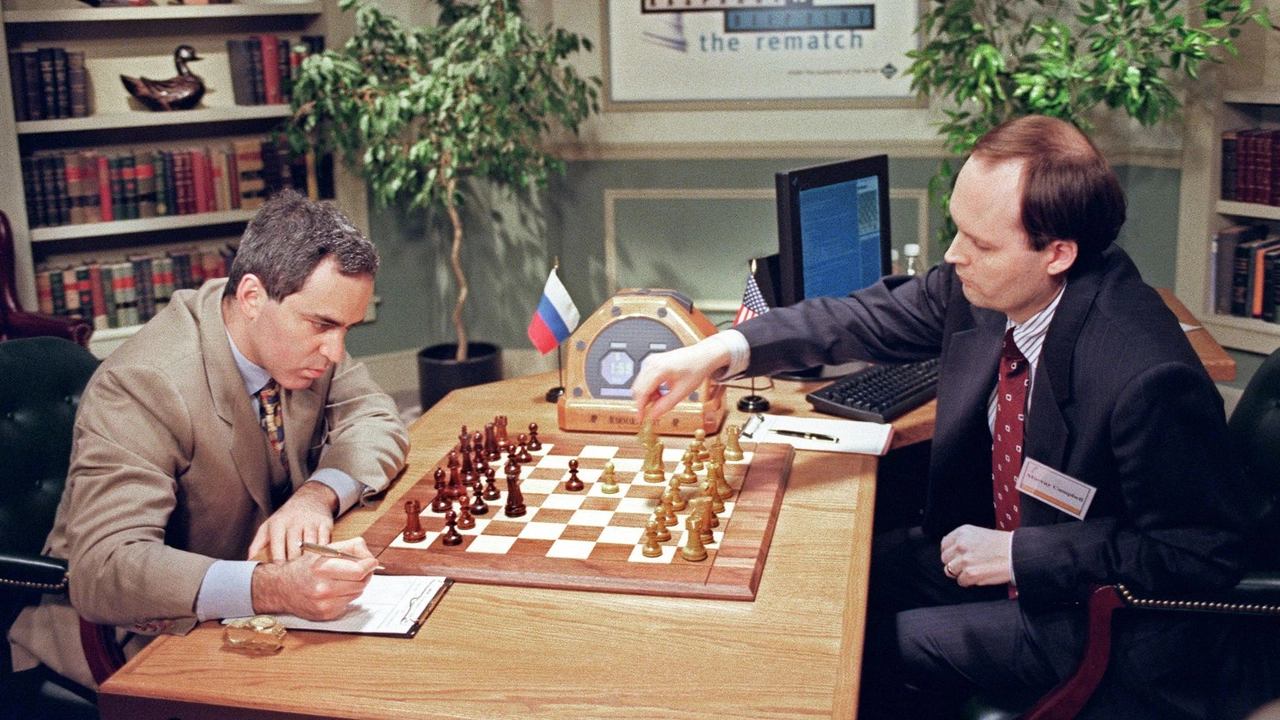
\includegraphics[width=0.8\textwidth]{figs/kasparovXdeepBlue.png} 
    
   Fonte: \cite{aibusiness2022deepblue}
\end{figure}

Com o advento de novas tecnologias, novas modalidades de jogos e desafios passaram a surgir, transformando e recriando clássicos dos jornais. Esses jogos passaram a mesclar inteligência artificial com semântica e exploração linguística, oferecendo novas perspectivas de como jogar. Um exemplo contemporâneo é o \textit{Contexto}\footnote{\url{https://contexto.me}, acessado em \today .}, um jogo online de adivinhação de palavras criado pelo programador Nildo Junior e disponível gratuitamente no navegador.

Inspirado no jogo norte-americano \textit{Semantle}, que utiliza \textit{word embeddings}, uma técnica de processamento de linguagem natural que transforma palavras em vetores numéricos, de forma que palavras com significados semelhantes fiquem próximas entre si no espaço vetorial \cite{mikolov2013efficient}, o Contexto desafia os jogadores a descobrirem a palavra secreta do dia com base em tentativas ilimitadas. A cada palpite, o jogo utiliza um algoritmo de IA para analisar a semelhança contextual entre a palavra sugerida e a palavra secreta, classificando-a em uma posição numérica. A palavra correta ocupa a posição número um, e quanto mais próxima dela estiver a tentativa do jogador, maior será sua pontuação. O sistema também recorre a cores para indicar a proximidade: vermelho para distante, amarelo para moderadamente próximo e verde para muito próximo.

O algoritmo do jogo foi treinado com milhares de textos em português, o que permite identificar palavras utilizadas em contextos semelhantes e calcular a proximidade semântica entre elas. A proposta de oferecer uma nova palavra diariamente incentiva a participação contínua dos jogadores, tornando o Contexto um exemplo atual de como os jogos, desde os tabuleiros do Egito até os navegadores modernos, continuam a evoluir com a tecnologia.

Modelos de IA são amplamente citados em livros, notícias e na literatura acadêmica, sendo utilizados como forma de desafiar o ser humano a ultrapassar seus próprios limites e também como ferramenta para aprimorar o desempenho. Assim, a busca por automatizar a resolução de jogos surge como uma maneira de explorar os limites da IA e, ao mesmo tempo, entender como ela pode nos desafiar. Nesse sentido, este trabalho propõe o desenvolvimento e a avaliação de um sistema automático capaz de resolver partidas do jogo Contexto utilizando modelos de word embeddings.

\section{Problemática}

Com o crescente interesse por jogos linguísticos mediados por IA, como Wordle e Contexto, surge uma nova fronteira de desafios computacionais: compreender o significado das palavras em seu contexto e simular o raciocínio humano na busca pela solução. No entanto, ainda são limitadas as soluções automatizadas eficazes, principalmente em idiomas como o português, que exigem nuances semânticas complexas. Diante disso, a problemática que se apresenta é desenvolver uma abordagem computacional capaz de automatizar a resolução de jogos de adivinhação de palavras em português, levando em consideração os desafios semânticos, contextuais e computacionais inerentes a essa tarefa. 

\section{Justificativa}

O avanço computacional tem possibilitado novas formas de interação homem-máquina, especialmente em domínios que envolvem linguagem natural. Jogos de adivinhação de palavras, como Contexto, têm se destacado por explorar relações semânticas complexas, representando uma oportunidade interessante para testar e aplicar modelos computacionais capazes de simular o raciocínio linguístico humano.

Apesar dos progressos em línguas como o inglês, a automatização desses jogos em português ainda é um campo pouco explorado, principalmente devido à escassez de recursos linguísticos e aos desafios semânticos próprios da língua. Desenvolver uma solução que consiga interpretar contextos, analisar similaridades e encontrar palavras de forma eficiente contribui não apenas para o avanço técnico da área, mas também para o fortalecimento de aplicações educacionais e recreativas com base em IA.

Este trabalho justifica-se pela relevância em propor uma abordagem que integre técnicas de processamento de linguagem natural, com foco na língua portuguesa, promovendo o desenvolvimento de soluções eficientes e adaptadas à nossa realidade linguística.
 
\section{Objetivo}

\subsection{ Objetivo Geral}

% Desenvolver uma abordagem computacional baseada em Inteligência Artificial capaz de automatizar a resolução de jogos de adivinhação de palavras em português, considerando aspectos semânticos, contextuais e computacionais da linguagem natural.

Desenvolver e avaliar um sistema automático capaz de resolver jogos de adivinhação de palavras, utilizando modelos de word embeddings pré-treinados, comparando o desempenho entre eles com base na taxa de acertos e no número de tentativas necessárias.

\subsection{Objetivos Específicos}

Considerando o desenvolvimento do trabalho e o objetivo geral apresentado, destacam-se os seguintes objetivos específicos:

% \begin{itemize}
%     \item Investigar os principais algoritmos e técnicas de \textit{Natural Language Processing} (NLP) aplicáveis à resolução de jogos de palavras;
%     \item Analisar o funcionamento de jogos como \textit{Contexto.me} e \textit{Semantle}, com foco nos critérios de similaridade semântica;
%     \item Implementar um modelo computacional que utilize representações vetoriais de palavras (\textit{word embeddings}) para simular tentativas em jogos de adivinhação;
%     \item Avaliar a eficácia da solução proposta com base na taxa de acertos e no número médio de tentativas;
%     \item Discutir os limites e as possibilidades da aplicação de IA em jogos linguísticos, especialmente no contexto da língua portuguesa.
% \end{itemize}

\begin{itemize}
    \item Desenvolver um sistema para a resolução automática de partidas do jogo Contexto;
    \item Implementar uma heurística de seleção de palavras capaz de conduzir o processo de busca pela palavra secreta;
    \item Avaliar a eficiência da heurística, utilizando métricas como taxa de acertos e número médio de tentativas para mensurar seu desempenho;
    \item Investigar diferentes modelos de word embeddings, compreendendo suas características e abordagens conceituais.
    \item Desenvolver um sistema que permita comparar o desempenho dos diferentes modelos de embeddings sob uma mesma heurística, garantindo uma análise comparativa consistente.
\end{itemize}

\section{Metodologia}

Para este trabalho, adotou-se o método de pesquisa exploratória, pois esse tipo de estudo visa proporcionar maior familiaridade com o problema, tornando-o mais explícito e auxiliando na formulação de hipóteses. O objetivo central da pesquisa é o aprimoramento de ideias ou a descoberta de novas intuições, sendo seu planejamento caracterizado por flexibilidade, o que permite a consideração de diferentes aspectos relacionados ao fenômeno estudado.

As pesquisas exploratórias normalmente envolvem levantamento bibliográfico, análise de exemplos que ampliem a compreensão do tema e entrevistas com especialistas na área. Neste trabalho, optou-se por concentrar a análise principalmente em fontes bibliográficas e exemplos relevantes, em conformidade com os objetivos da pesquisa e com a natureza exploratória do estudo.


\section{Organização}
O presente trabalho está organizado da seguinte forma:

O \textbf{Capítulo 1} apresenta a introdução do estudo, contextualizando o problema de pesquisa, sua relevância no cenário atual, os objetivos gerais e específicos, bem como a metodologia empregada.

O \textbf{Capítulo 2} trata dos trabalhos relacionados, reunindo estudos e projetos previamente desenvolvidos que possuem afinidade com o tema abordado, a fim de embasar teoricamente a proposta.

O \textbf{Capítulo 3} aborda os principais conceitos, fundamentos e ferramentas envolvidos na execução do projeto, detalhando os elementos que sustentam a construção da proposta.

O \textbf{Capítulo 4} descreve o desenvolvimento da solução proposta, detalhando as etapas e processos adotados na implementação e na construção da resolução de jogos de adivinhar palavras.

O \textbf{Capítulo 5} apresenta as considerações finais, destacando os resultados obtidos, as contribuições do trabalho e sugestões para futuras melhorias e desdobramentos do projeto.
\chapter{Referencial Teórico}

Este capítulo reúne os fundamentos conceituais que sustentam a proposta do chatbot financeiro, contemplando soluções correlatas e as principais tecnologias empregadas na construção do sistema.

\section{Trabalhos Relacionados}

O levantamento de trabalhos relacionados tem como objetivo identificar abordagens já utilizadas em soluções de automação conversacional, controle financeiro digital e integração entre assistentes virtuais e plataformas de mensageria. Essa análise permite compreender práticas adotadas no mercado e na literatura, bem como delimitar o diferencial da proposta desenvolvida neste trabalho.

\subsection{Concorrentes}

Entre as soluções concorrentes, destacam-se aplicativos de gestão financeira que oferecem categorização de despesas, relatórios e metas, além de assistentes conversacionais voltados a atendimento automatizado. De modo geral, essas ferramentas evidenciam a importância da usabilidade, da integração com canais familiares e da apresentação clara de indicadores financeiros. Como texto-base provisório, esta subseção deverá ser refinada com a descrição comparativa de produtos específicos e suas funcionalidades.

\subsection{Artigos Científicos Relacionados}

Na literatura científica, estudos sobre chatbots, interfaces conversacionais e apoio à tomada de decisão mostram que sistemas baseados em linguagem natural podem reduzir barreiras de uso e aumentar a frequência de interação dos usuários com serviços digitais. Para a versão final do trabalho, esta subseção deverá incorporar referências bibliográficas que abordem chatbots financeiros, interação humano-computador, adoção de mensageria e recomendação personalizada em contexto financeiro.

\section{Tecnologias}

As tecnologias selecionadas para a solução foram escolhidas com base em integração, facilidade de automação, escalabilidade e aderência ao fluxo proposto para o produto.

\subsection{WhatsApp}

O WhatsApp será utilizado como principal canal de interação com o usuário. A escolha dessa plataforma se justifica por sua ampla adoção, familiaridade de uso e capacidade de reduzir a fricção no registro de informações do dia a dia. No contexto da solução, o aplicativo funciona como porta de entrada para mensagens, comandos, alertas e confirmações de lançamentos financeiros.

\subsection{Evolution API}

A Evolution API atua como camada de integração entre o sistema proposto e o WhatsApp, permitindo o envio e recebimento de mensagens, além da orquestração de eventos conversacionais. Nesta etapa do trabalho, a subseção registra seu papel arquitetural e deverá ser expandida posteriormente com detalhes de autenticação, webhooks e fluxo de mensagens.

\subsection{Chatbot}

O chatbot representa o núcleo conversacional da solução, sendo responsável por interpretar mensagens em linguagem natural, direcionar o fluxo de atendimento e acionar os serviços internos necessários ao registro e à consulta de dados financeiros. Sua modelagem considera clareza de resposta, simplicidade operacional e contextualização adequada para o usuário final.

\subsection{n8n}

O n8n será empregado como ferramenta de automação para integrar etapas do fluxo conversacional, regras de negócio e serviços externos. Seu uso favorece a criação de rotinas visuais de processamento, reduzindo o acoplamento direto entre todas as integrações e permitindo maior flexibilidade na manutenção dos fluxos.

\subsection{Groq API}

A Groq API é considerada na proposta como serviço de apoio ao processamento de linguagem natural, com potencial para interpretar intenções, estruturar informações extraídas das mensagens e apoiar respostas contextualizadas. Esta subseção permanece como base conceitual e deverá ser aprofundada na versão final com a estratégia de uso da API na arquitetura.

\subsection{Docker}

O Docker será utilizado para padronizar a execução dos serviços da aplicação em ambientes isolados, favorecendo reprodutibilidade e portabilidade. Seu uso contribui para simplificar a configuração do ambiente de desenvolvimento e implantação da solução.

\subsection{Docker Compose}

O Docker Compose será empregado para orquestrar os contêineres necessários ao funcionamento do sistema, como backend, automação, banco de dados e interface web. A adoção dessa ferramenta permite definir e subir a infraestrutura local de forma integrada.

\subsection{React}

O React será utilizado na construção da interface web destinada à visualização de relatórios, gráficos e dados financeiros consolidados. A escolha se deve à flexibilidade para composição de componentes e à facilidade de criação de interfaces dinâmicas voltadas à experiência do usuário.

\subsection{PostgreSQL}

O PostgreSQL será o sistema de gerenciamento de banco de dados da aplicação, responsável por persistir usuários, lançamentos financeiros, categorias, metas e demais entidades necessárias ao funcionamento da solução. Sua adoção se justifica pela robustez, confiabilidade e aderência a aplicações transacionais.

\chapter{Gestão dos Conhecimentos}

Neste capítulo, serão apresentadas as tecnologias que serão utilizadas para o desenvolvimento do projeto, e o motivo da utilização, além de uma contextualização de cada uma delas.

% \section{Machine Learning}

% \textit{Machine Learning} é uma área da Ciência da Computação que estuda o desenvolvimento de algoritmos capazes de aprender a executar uma tarefa com sua própria experiência, sem
% a necessidade de programar explicitamente todas as regras para cada tarefa específica \cite{cerri2019aprendizado}. A complexidade do aprendizado de máquina reside no fato de que o sucesso dos algoritmos depende da qualidade e da quantidade dos dados, além da escolha adequada dos modelos e técnicas \cite{DBLP:journals/cacm/Domingos12}.

% Existem três principais paradigmas em aprendizado de máquina: Aprendizado Supervisionado, Não Supervisionado e por Reforço.

% No Aprendizado Supervisionado, o modelo é treinado com dados rotulados, onde, para cada exemplo apresentado ao algoritmo, há uma resposta correta associada. Nesse caso, o algoritmo aprende a relacionar entradas às saídas desejadas, buscando generalizar esse conhecimento para realizar previsões precisas sobre novos dados.

% Por outro lado, no Aprendizado Não Supervisionado, os dados fornecidos ao algoritmo não possuem rótulos. O objetivo é identificar padrões ou estruturas ocultas nos exemplos sem orientação explícita. Algoritmos comuns buscam agrupar dados semelhantes, formando agrupamentos ou \textit{clusters}.

% Já no Aprendizado por Reforço, o algoritmo interage diretamente com um ambiente, recebendo recompensas ou punições conforme suas ações. As recompensas reforçam comportamentos desejáveis, enquanto as punições servem para impedir as ações fracassadas. O objetivo é maximizar a recompensa acumulada ao longo do tempo, desenvolvendo uma política ótima de comportamento. O algoritmo \textit{Q-Learning} é um dos mais conhecidos e utilizados desse paradigma \cite{watkins1989learning}.

% É importante levantar que os modelos de Processamento de Linguagem Natural abordados neste trabalho, como o GloVe e o FastText, utilizam o aprendizado não supervisionado para seu treinamento.

\section{Word Embeddings}

No processamento de linguagem natural, word embeddings são representações vetoriais que mapeiam palavras para um conjunto de vetores de valores reais em um espaço N-dimensional predefinido, de modo que palavras que possuem significado semântico, contextual e sintático próximas no vocabulário sejam representadas por vetores próximos nesse espaço \cite{mikolov2013efficient}. Essas representações são aprendidas por meio de algoritmos de \textit{machine learning} que são gerados a partir de seu contexto.

\begin{figure}[h!]
    \centering
    
    \label{fig:relacao-lineares-palavras}
    \caption{Relações lineares entre palavras.}
    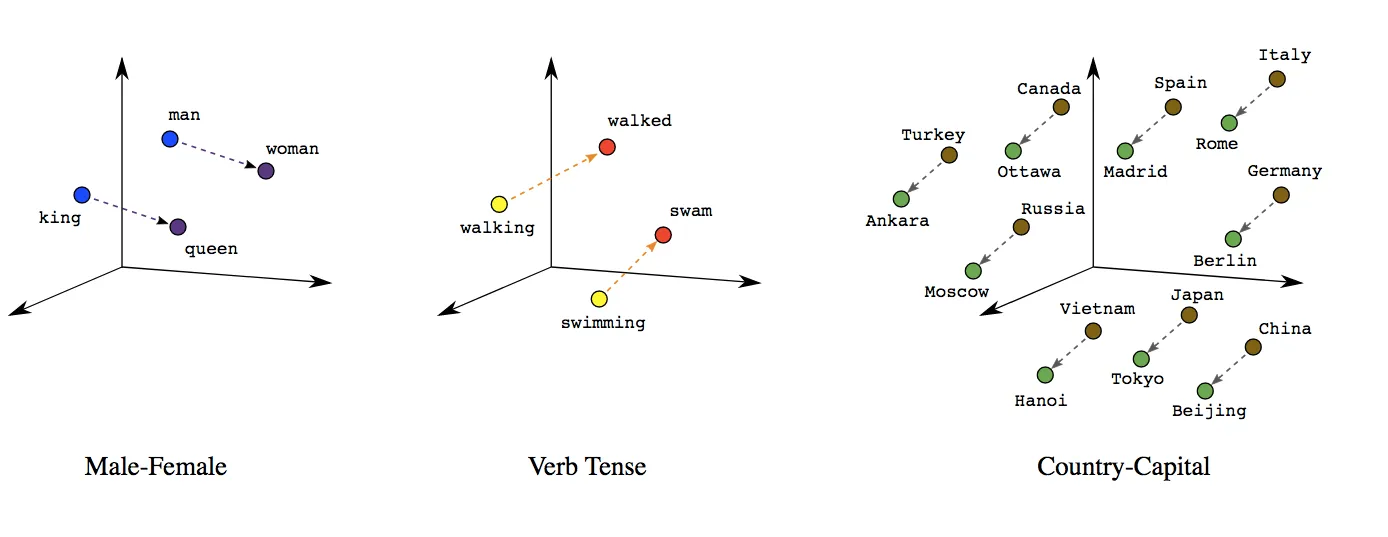
\includegraphics[width=1\textwidth]{figs/relacao-palavras.jpg} 
    
    Fonte: \cite{duzzi2023}
\end{figure}

Inicialmente, técnicas como \textit{Bag of Words} (BoW) e TF-IDF eram amplamente utilizadas, baseando-se em vetores de alta dimensionalidade, nos quais cada palavra era representada como um índice isolado, sem considerar semelhanças semânticas entre diferentes termos. Apesar de sua simplicidade, esses métodos apresentavam limitações expressivas, especialmente na incapacidade de capturar relações semânticas ou contextuais entre as palavras \cite{mikolov2013efficient}.

Existem diversas abordagens para a obtenção de representações vetoriais de palavras, mas a maneira mais popular é treinando redes neurais, como é o caso do famoso \textit{Word2vec}, modelo de aprendizado de máquina desenvolvido por \citeonline{mikolov2013efficient} em 2013. Esse algoritmo utiliza redes neurais rasas para gerar embeddings.

\section{Word2Vec}

O modelo Word2Vec pode ser treinado a partir de duas arquiteturas possíveis: \textit{Continuous Bag-of-Words} (CBOW) e \textit{Skip-Gram}. O CBOW prevê uma palavra com base em seu contexto, enquanto o Skip-Gram prevê o contexto a partir de uma palavra. Por exemplo, a expressão vetorial “vetor(‘rei’) - vetor(‘homem’) + vetor(‘mulher’)” resulta em um vetor próximo ao vetor de “rainha”, evidenciando a captura das relações semânticas \cite{MikolovYZ13}.

A arquitetura do Word2Vec é baseada em uma rede neural rasa composta por três camadas: entrada, oculta e saída. Na camada de entrada, cada palavra é representada por um vetor one-hot, que é então transformado em um vetor denso na camada oculta por meio de uma matriz de pesos. Essa matriz de pesos é, na verdade, o que constitui os embeddings de palavras aprendidos pelo modelo \cite{Rong14}.

\begin{figure}[h!]
    \centering
    
    \label{fig:representacao-modelos-w2v}
    \caption{Representação dos modelos Word2Vec.}
    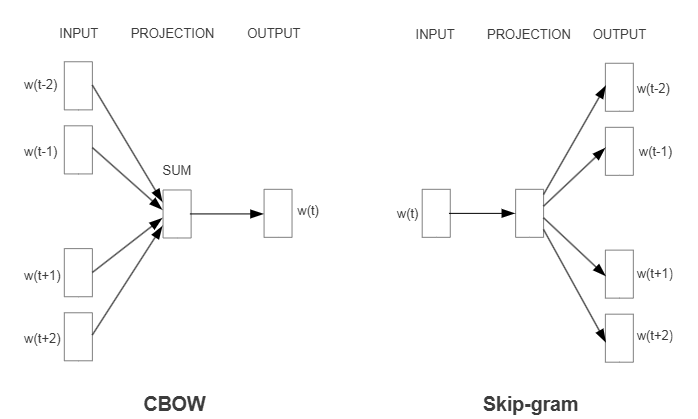
\includegraphics[width=1\textwidth]{figs/representacao-modelos-w2v.png} 
    
    Fonte: \cite{mikolov2013efficient}
\end{figure}

Já a camada de saída utiliza outra matriz de pesos para prever as palavras de contexto, no modelo Skip-Gram, ou a palavra central, no modelo CBOW, aplicando uma função \textit{softmax} para gerar uma distribuição de probabilidade sobre o vocabulário. O treinamento da rede ajusta os pesos de ambas as matrizes para minimizar a diferença entre as previsões e as palavras reais observadas no corpus.

\section{GloVe}

O \textit{GloVe}, sigla para \textit{Global Vectors } (Vetores Globais), desenvolvido per \citeonline{pennington2014glove}, é um algoritmo de aprendizado não supervisionado usado para criar word embeddings. Sua principal inovação foi combinar o melhor de duas abordagens anteriores: a eficiência estatística global dos métodos baseados em contagem, como a análise de coocorrência em todo o texto, e o desempenho superior em tarefas de analogia dos métodos preditivos baseados em contexto local, como o Word2Vec.

O GloVe opera construindo uma matriz global de coocorrência de palavras e, em seguida, treina um modelo de regressão ponderada para aprender vetores cujo produto escalar se aproxima do logaritmo da probabilidade de coocorrência dessas palavras. O resultado são embeddings que capturam de forma eficaz as relações semânticas e sintáticas complexas.

\section{FastText}

Técnicas de incorporação de palavras, como Word2Vec e GloVe, fornecem representações vetoriais únicas para cada palavra do vocabulário, negligenciando a estrutura morfológica interna desses termos. Essa abordagem é uma limitação significativa para línguas morfologicamente ricas, pois ignora as relações sintáticas e semânticas evidentes na formação das palavras (prefixos, sufixos e radicais).

Para superar essa limitação, o \textit{FastText}, uma extensão do modelo Word2Vec, enriquece as representações vetoriais usando informações em nível de caractere. O FastText aprende embeddings para n-gramas de caracteres (subpartes da palavra) e representa uma palavra como a soma ou a média dos vetores de seus n-gramas constituintes. Assim como o antecessor, ele também utiliza as arquiteturas CBOW e Skip-Gram para o treinamento.

A principal vantagem dessa abordagem é a capacidade de lidar com palavras fora do vocabulário (\textit{Out-of-Vocabulary} — OOV). Modelos como Word2Vec ou GloVe não conseguem gerar vetores para palavras que não estavam presentes nos dados de treinamento. O FastText, ao contrário, pode construir a representação de uma palavra OOV simplesmente somando os vetores de seus n-gramas de caracteres, permitindo-lhe inferir o significado de termos novos ou raros com base em sua composição. \cite{bojanowski-etal-2017-enriching}

\section{Tecnologias}

\subsection{Python}

\textit{Python} é uma linguagem de programação de alto nível, criada por Guido van Rossum em fevereiro de 1991. A linguagem foi desenvolvida com uma sintaxe clara e legível, que se assemelha à linguagem humana. Além disso, o Python é uma linguagem interpretada e de tipagem dinâmica, o que significa que as variáveis não precisam ter seu tipo explicitamente declarado, facilitando a curva de aprendizado e o desenvolvimento de aplicações.

Em 2024, Python se tornou a linguagem de programação mais utilizada no \textit{GitHub}, ultrapassando \textit{JavaScript} pela primeira vez desde o início da plataforma\footnote{\url{https://github.blog/news-insights/octoverse/octoverse-2024/}, acessado em \today.}. Essa marca só foi possível de ser alcançada devido ao aumento de projetos relacionados à Inteligência Artificial, ciência de dados e aprendizado de máquina, áreas nas quais Python é amplamente adotado devido à extensa variedade de bibliotecas disponíveis. 

% Por esse mesmo motivo, Python foi escolhido como a linguagem de programação para este projeto, garantindo uma implementação alinhada com as tendências atuais do desenvolvimento de aprendizado de máquina.

\subsection{Gensim}

O \textit{Gensim} é uma biblioteca \textit{open-source} em Python projetada para representar documentos como vetores semânticos de maneira eficiente, facilitando o processamento e análise de textos não estruturados. Utilizando algoritmos de aprendizado não supervisionado, como Word2Vec e FastText, o Gensim é capaz de descobrir automaticamente a estrutura semântica dos documentos, analisando padrões de coocorrência estatística em grandes corpora de texto. Esses modelos transformam textos em representações vetoriais, permitindo consultas de similaridade semântica entre palavras, frases e documentos, o que promove uma análise mais profunda e automatizada do conteúdo textual. \cite{rehurek_lrec}

% O Gensim foi utilizado no projeto para carregar o modelo de embending e fazer as comparações.

\subsection{Playwright}
O \textit{Playwright} é um framework de código aberto mantido pela \textit{Microsoft}, desenvolvido para a automação de navegadores e a execução de testes de ponta-a-ponta (\textit{end-to-end}). Seu principal diferencial é a capacidade de controlar os três principais motores de renderização, \textit{Chromium}, \textit{Firefox} e \textit{WebKit}, por meio de uma API única e unificada. Essa abordagem permite que desenvolvedores e analistas de qualidade escrevam um único \textit{script} de teste e o executem de forma consistente em todos os principais navegadores. O framework oferece suporte a diversas linguagens, como Python, JavaScript, Java e C\#.\footnote{\url{https://playwright.dev/docs/intro}, acessado em \today.}

% \subsection{Numpy}
% NumPy é o pacote fundamental para computação científica em Python. É uma biblioteca Python que fornece um objeto de array multidimensional, vários objetos derivados (como arrays e matrizes mascaradas) e uma variedade de rotinas para operações rápidas em arrays, incluindo operações matemáticas, lógicas, manipulação de formas, ordenação, seleção, entrada/saída, transformadas discretas de Fourier, álgebra linear básica, operações estatísticas básicas, simulação aleatória e muito mais.\footnote{\url{https://numpy.org/doc/stable}, acessado em \today.

\subsection{Hugging Face Hub}
O Hugging Face Hub é uma plataforma com mais de 2 milhões de modelos, 500 mil conjuntos de dados e 1 milhão de demonstrações, na qual as pessoas podem colaborar facilmente em seus fluxos de trabalho de aprendizado de máquina. O Hub funciona como um local central onde qualquer pessoa pode compartilhar, explorar, descobrir e experimentar com aprendizado de máquina de código aberto.\footnote{\url{https://huggingface.co/docs/hub/index}, acessado em \today.}
\chapter{Proposta de Solução}

Este capítulo apresenta a proposta de solução para o problema investigado, descrevendo a documentação técnica inicial do sistema, os requisitos identificados, os principais artefatos de modelagem e a visão geral do protótipo.

\section{Documentação Técnica}

A documentação técnica da solução tem como objetivo organizar, de forma estruturada, as decisões relacionadas ao funcionamento do sistema, às integrações previstas e ao comportamento esperado da aplicação. Nesta etapa, a documentação cumpre o papel de consolidar os resultados da pesquisa com usuários e transformá-los em especificações iniciais para desenvolvimento.

\subsection{Levantamento de Requisitos}

O levantamento de requisitos foi orientado pelos achados da pesquisa qualitativa e pelas histórias de usuário definidas no capítulo anterior. A seguir, são apresentados requisitos iniciais que servirão de base para o detalhamento técnico da solução.

\subsubsection{Requisitos Funcionais}

\begin{itemize}
    \item O sistema deve interpretar e processar mensagens enviadas pelo usuário via WhatsApp utilizando Inteligência Artificial.
    \item O sistema deve identificar automaticamente os valores, tipos de movimentação (receita/despesa) e categorias presentes nas mensagens de linguagem natural do usuário.
    \item O sistema deve gerar gráficos financeiros com base nos dados registrados pelo usuário.
    \item O sistema deve permitir que o usuário possa se cadastrar.
    \item O sistema deve permitir que o usuário faça o login, baseado nos dados cadastrados.
    \item O sistema deve ter uma visualização web, que permita ao usuário ver os dashboards criados.
    \item O sistema deve permitir separar gastos por categorias.
    \item O sistema deve permitir a configuração do estilo de comunicação do assistente virtual conforme a preferência do usuário.
    \item O sistema deve permitir que o usuário reserve valores para metas financeiras específicas, desconsiderando-os do saldo disponível.
    \item O sistema deve permitir que o usuário edite as movimentações financeiras registradas.
    \item O sistema deve permitir que o usuário remova as movimentações financeiras registradas.
    \item O sistema deve permitir a geração de relatórios financeiros com base nos dados registrados pelo usuário.
    \item O sistema deve permitir que o usuário exporte o relatório para fora do site.
    \item O assistente de IA deve manter o contexto da conversa com o usuário, permitindo interações contínuas e mais fluidas.
\end{itemize}

\subsubsection{Requisitos Não Funcionais}

\begin{itemize}
    \item O sistema deve apresentar fluxo de uso simples, intuitivo e compatível com usuários sem conhecimento técnico.
    \item O processo de registro financeiro deve exigir o menor número de etapas, reduzindo o esforço necessário para utilização contínua da plataforma.
    \item A interface conversacional deve utilizar linguagem clara, objetiva e de fácil compreensão para o usuário.
    \item O sistema deve permitir utilização em dispositivos móveis, considerando que o WhatsApp será o principal canal de interação.
    \item O sistema deve garantir persistência, integridade e segurança dos dados financeiros registrados pelos usuários.
    \item A solução deve possuir arquitetura modular, permitindo evolução futura das integrações e funcionalidades.
    \item A aplicação deve ser coerente com execução em ambiente conteinerizado utilizando Docker.
    \item O dashboard web deve apresentar informações financeiras de forma visual, organizada e acessível.
    \item O sistema deve priorizar facilidade de uso e baixo esforço mental, buscando incentivar constância no acompanhamento financeiro.
    \item O sistema deve oferecer experiência coerente com a rotina do dia a dia do usuário, permitindo registros rápidos por linguagem natural.
\end{itemize}

\subsection{Modelagem}

A modelagem do sistema possui papel fundamental no processo de desenvolvimento de software, pois permite representar de forma visual a estrutura, os componentes e os relacionamentos existentes na aplicação antes de sua implementação. Por meio da modelagem, torna-se possível compreender melhor o funcionamento do sistema, organizar os requisitos levantados e facilitar a comunicação entre os integrantes do projeto. Além disso, os modelos desenvolvidos auxiliam na documentação da aplicação, contribuindo para o planejamento da arquitetura do software e para a definição das regras de negócio envolvidas no sistema.

No contexto da presente proposta, a modelagem foi utilizada para representar os principais elementos, para isso, foram elaborados diagramas voltados à representação estrutural e organizacional da aplicação, permitindo visualizar os componentes principais. Dessa forma, a modelagem contribui para demonstrar como os elementos do sistema se relacionam, além de servir como apoio para o desenvolvimento da solução proposta.

\subsubsection{Diagrama de Casos de Uso}

O diagrama de casos de uso consiste em uma representação da UML utilizada para apresentar, de maneira visual, as principais funcionalidades oferecidas por um sistema e as interações estabelecidas entre essas funcionalidades e seus atores. Os atores correspondem a usuários, sistemas externos ou outras entidades que se relacionam com o sistema, enquanto os casos de uso representam ações, processos ou objetivos que podem ser executados. Esse tipo de diagrama assume papel relevante nas etapas de levantamento e modelagem de requisitos, uma vez que contribui para a delimitação do escopo do sistema, para a identificação de suas funcionalidades centrais e para a facilitação da comunicação entre desenvolvedores, orientadores e demais envolvidos no projeto.

No diagrama de casos de uso desenvolvido para a proposta deste trabalho, o ator principal é o Usuário, responsável por interagir com o sistema para registrar transações financeiras por meio do WhatsApp, consultar saldo, acessar relatórios financeiros, cadastrar e acompanhar metas, visualizar o dashboard web e receber alertas financeiros. O diagrama também contempla funcionalidades internas necessárias ao funcionamento da solução, tais como interpretar linguagem natural, classificar transações, confirmar registros financeiros, identificar gastos recorrentes, gerar recomendações personalizadas, emitir relatórios e armazenar dados financeiros.

\begin{figure}[H]
    \centering
    \caption{Diagrama de casos de uso da solução proposta}
    \label{fig:diagrama-casos-uso}
    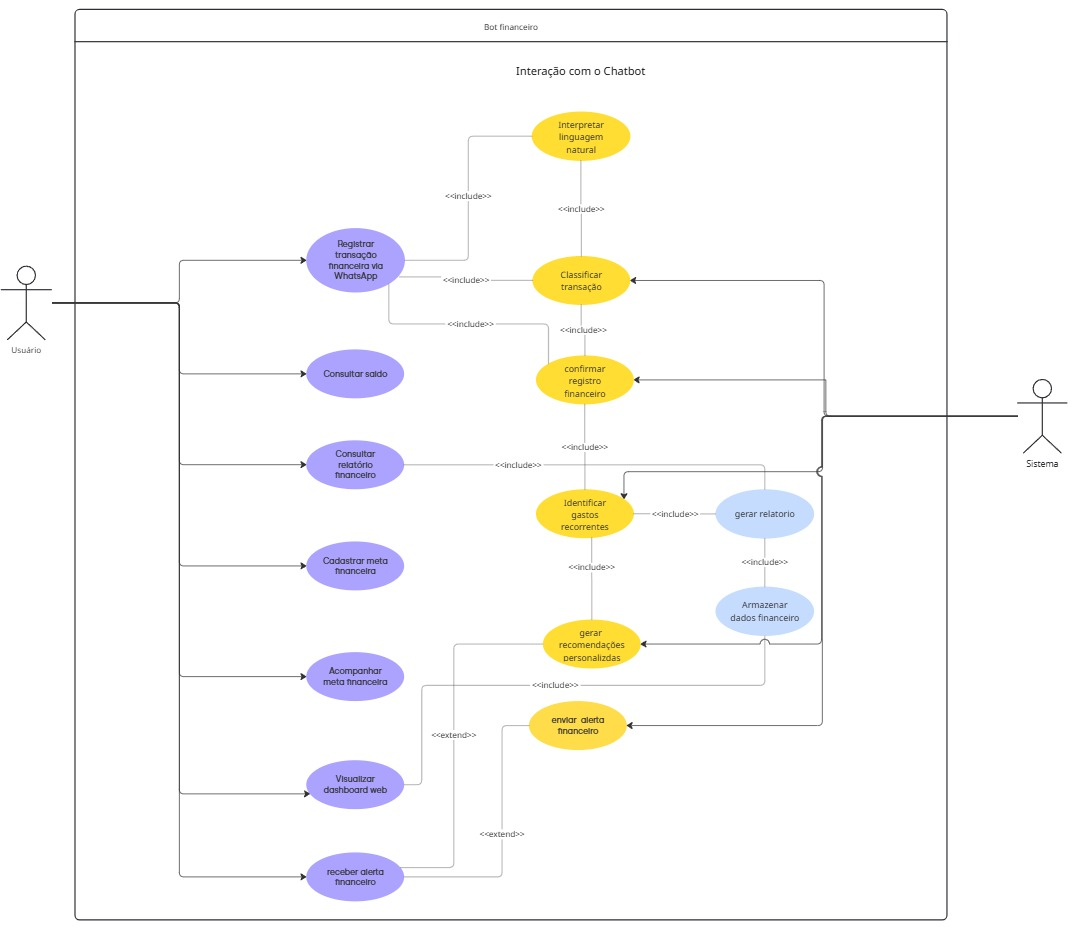
\includegraphics[width=\textwidth]{figs/diagrama-caso-de-uso.png}
    \fonte{Elaborado pelos autores.}
\end{figure}

\subsubsection{Diagrama de Classes}

O diagrama de classes é um dos diagramas mais utilizados da UML, sendo responsável por representar a estrutura estática de um sistema orientado a objetos. Esse tipo de diagrama permite demonstrar as classes existentes no sistema, seus atributos, métodos e os relacionamentos entre elas. Além disso, o diagrama de classes auxilia na visualização da organização do software, contribuindo para a compreensão da arquitetura do sistema e das responsabilidades de cada componente.

No contexto da presente proposta, o diagrama de classes contempla as entidades centrais pelo gerenciamento de usuários, mensagens, transações financeiras, categorias, metas financeiras e notificações. Além disso, o diagrama também apresenta uma classe de serviço responsável pelas funcionalidades de inteligência artificial, incluindo processamento de mensagens, geração de recomendações e emissão de alertas financeiros. Os relacionamentos apresentados demonstram como os componentes do sistema se conectam, permitindo a integração entre o controle financeiro, a comunicação conversacional e os recursos inteligentes propostos pela aplicação.

\begin{figure}[H]
    \centering
    \caption{Diagrama de classes}
    \label{fig:diagrama-classes}
    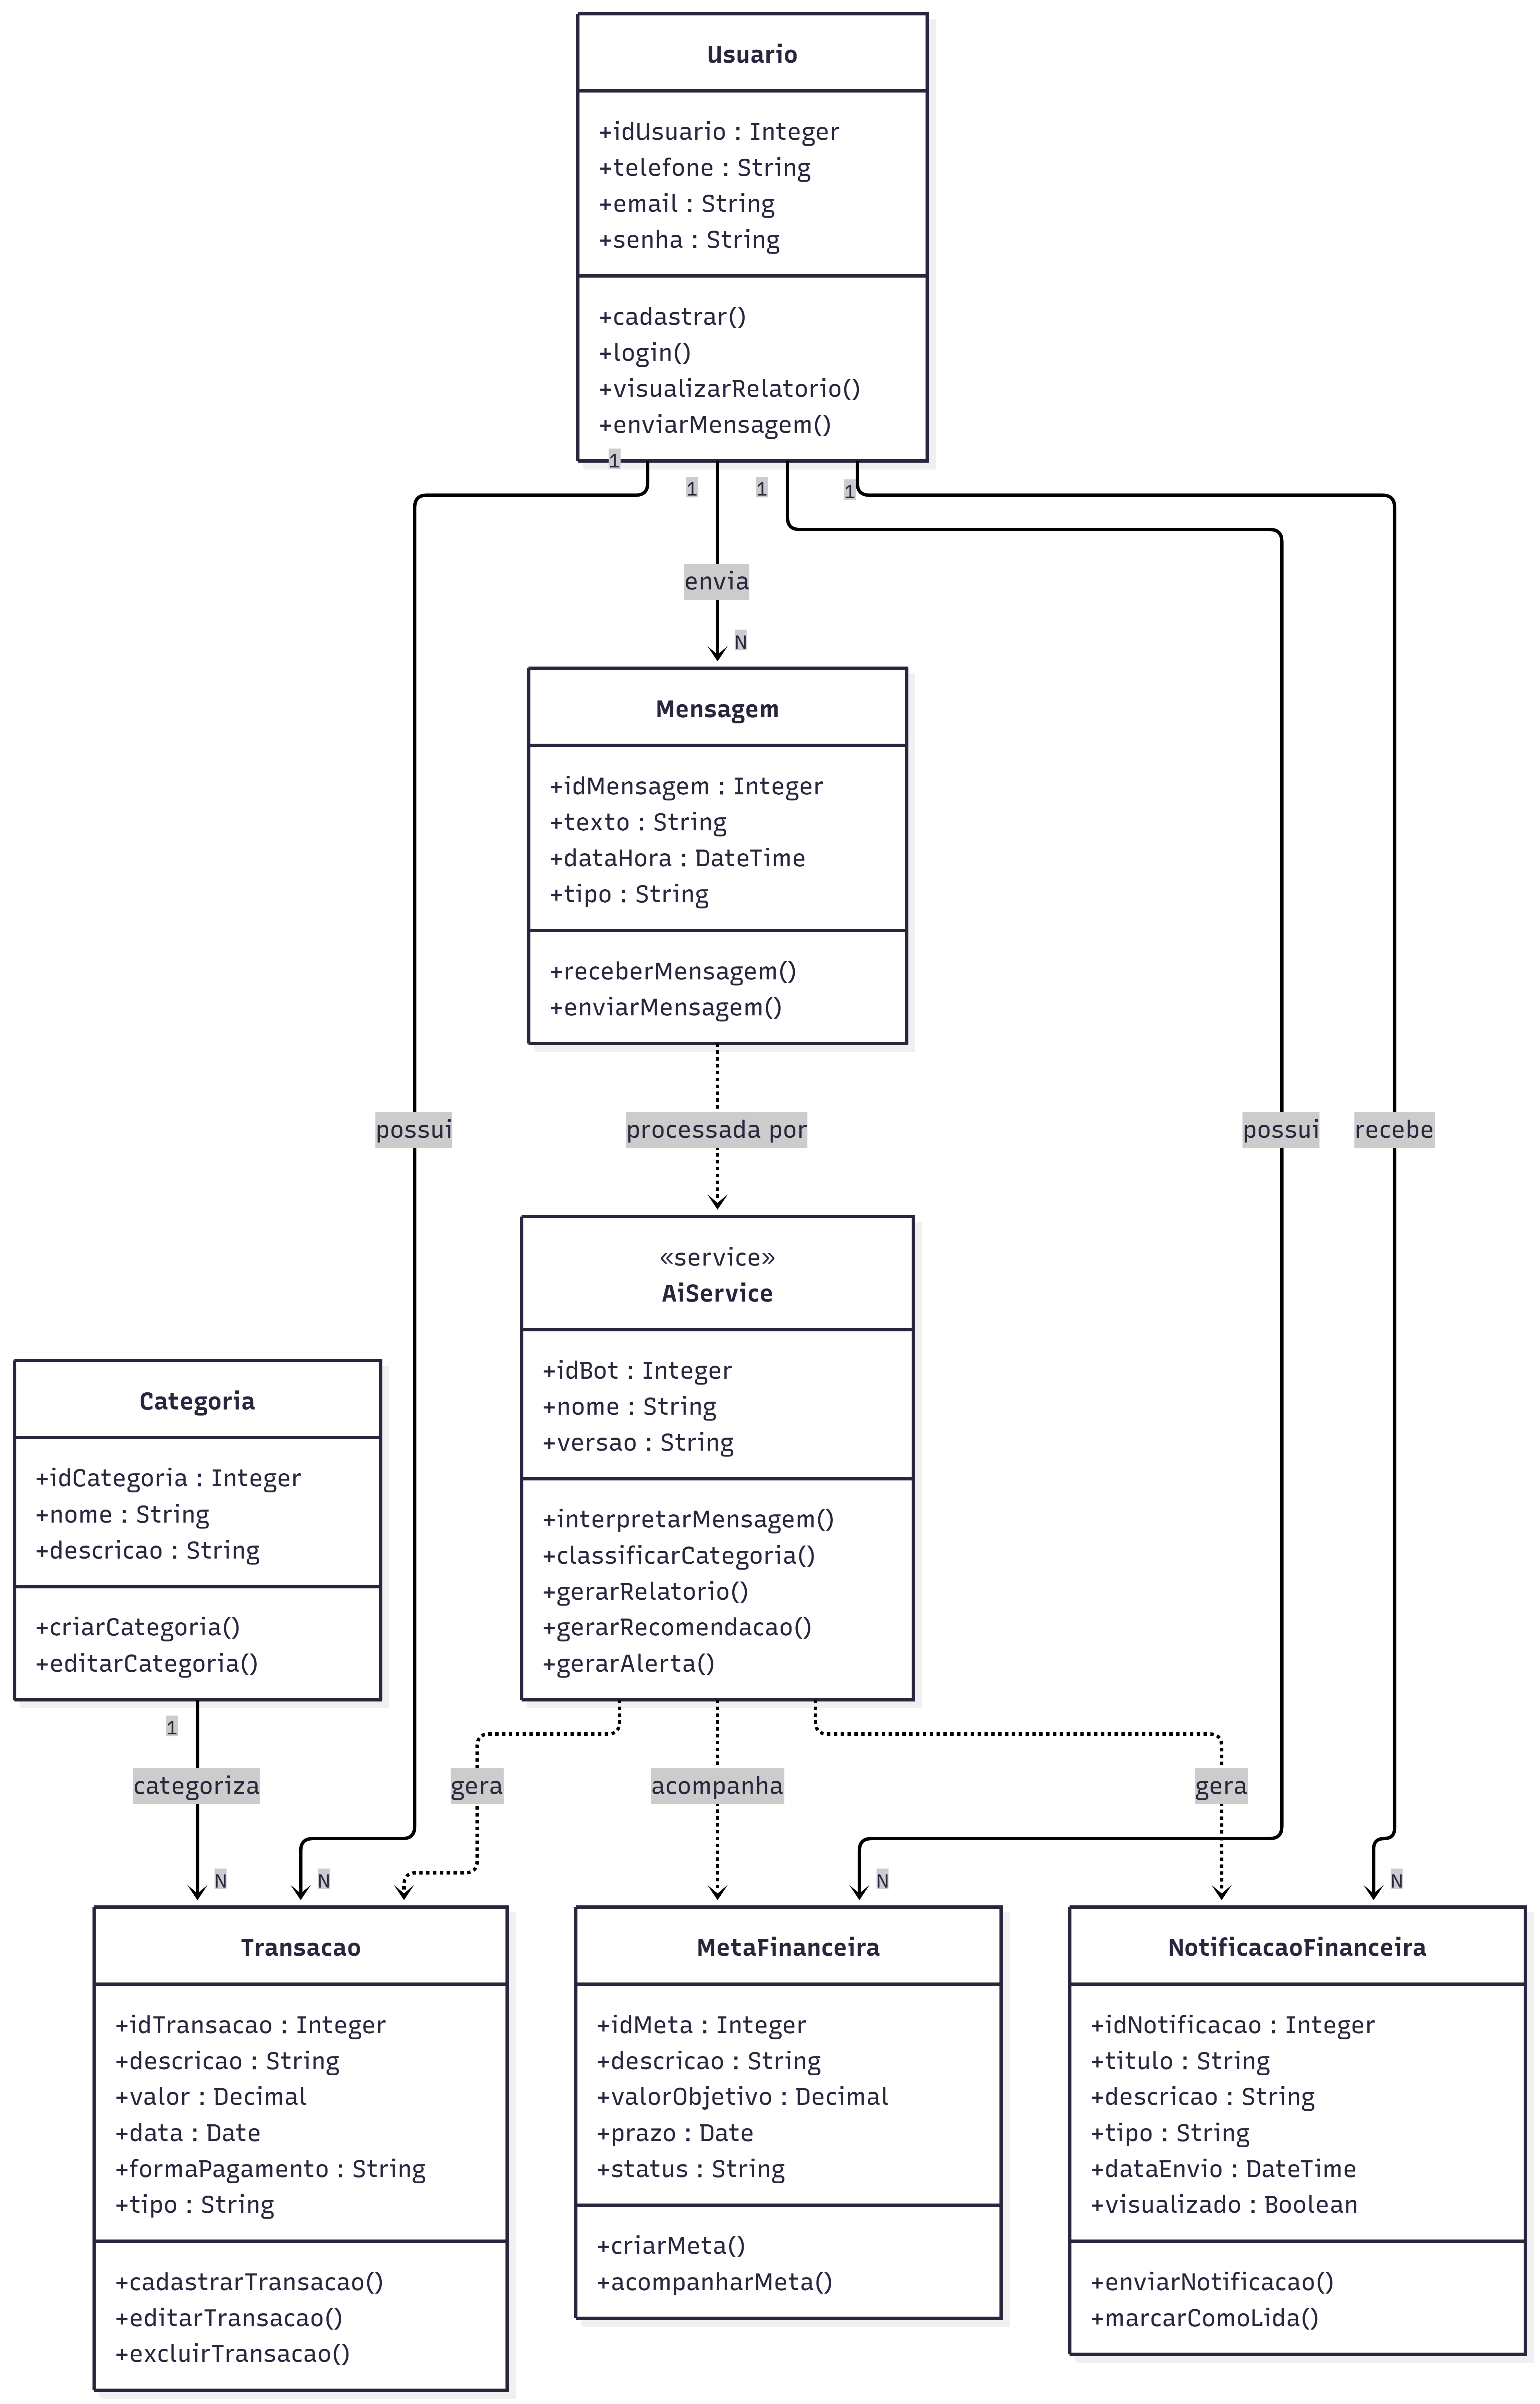
\includegraphics[width=0.8\textwidth]{figs/diagrama-de-classe.png}
    \fonte{Elaborado pelos autores.}
\end{figure}

\subsubsection{Diagrama Entidade-Relacionamento}

O diagrama entidade-relacionamento é uma técnica de modelagem utilizada para representar a estrutura lógica de um banco de dados, permitindo visualizar entidades, atributos e os relacionamentos existentes entre os dados do sistema. Esse tipo de diagrama auxilia na organização e no planejamento do banco de dados, contribuindo para a definição das informações que serão armazenadas e da forma como essas informações se relacionam dentro da aplicação. Além disso, o modelo entidade-relacionamento é amplamente utilizado durante o desenvolvimento de sistemas para facilitar a compreensão da estrutura dos dados e apoiar a implementação do banco de dados.

No contexto da presente proposta, o diagrama entidade-relacionamento representa as principais entidades relacionadas ao gerenciamento financeiro e à comunicação conversacional do sistema. A estrutura contempla entidades responsáveis pelo armazenamento de usuários, conversas, mensagens, transações financeiras, categorias, metas financeiras e notificações. Os relacionamentos apresentados demonstram como essas entidades se conectam dentro do banco de dados, permitindo o gerenciamento das informações financeiras, o armazenamento do histórico de conversas e o envio de notificações ao usuário. Dessa forma, o diagrama evidencia a organização dos dados necessários para o funcionamento da aplicação proposta.

\begin{figure}[H]
    \centering
    \caption{Diagrama entidade-relacionamento}
    \label{fig:diagrama-erd}
    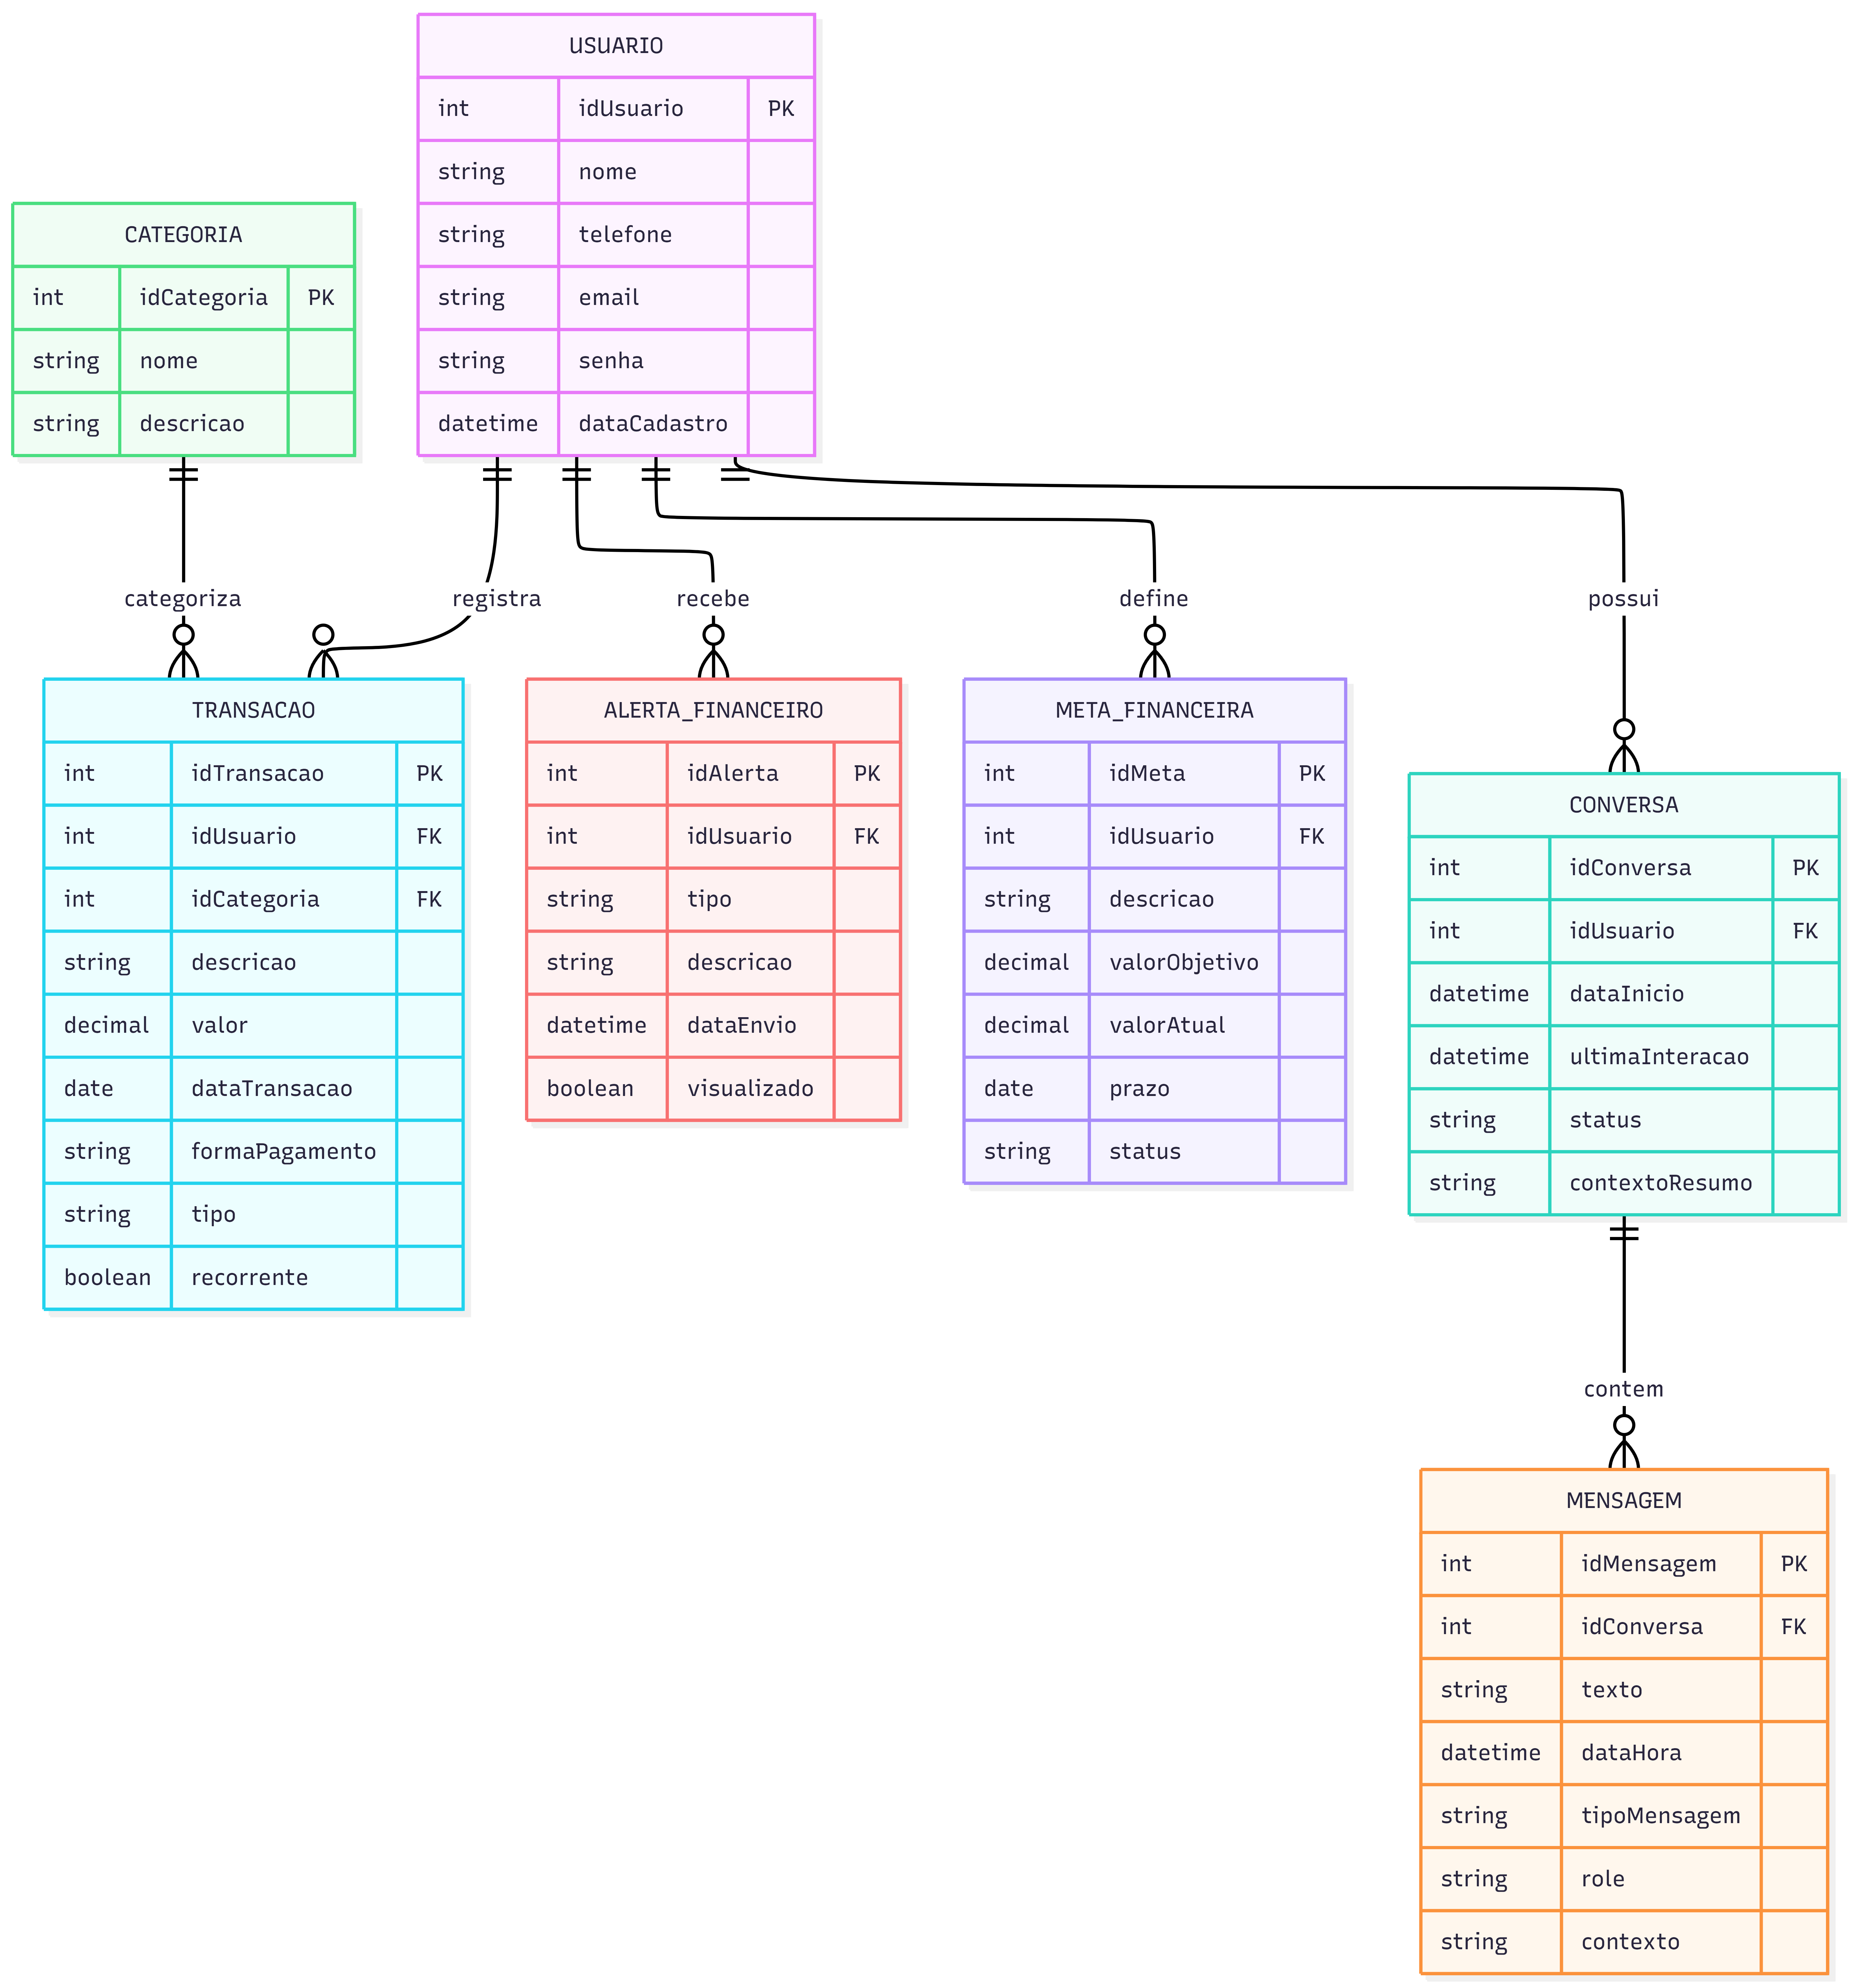
\includegraphics[width=0.8\textwidth]{figs/diagrama-entidade-relacionamento.png}
    \fonte{Elaborado pelos autores.}
\end{figure}

\subsection{Protótipo da Interface de Usuário}

O protótipo da solução contempla dois eixos principais: a experiência conversacional no WhatsApp e a interface web para visualização de dashboards e relatórios. A proposta busca oferecer uma jornada de usuário fluida, começando pelo registro simplificado de gastos via linguagem natural e culminando em uma análise visual completa da saúde financeira.

\subsubsection{Fluxo de cadastro e uso do sistema}

O uso da solução proposta pode começar por dois caminhos. No primeiro, o usuário acessa diretamente a versão web do GranaAI, abre a tela de cadastro e preenche as informações solicitadas pelo sistema. Após a conclusão do formulário, a plataforma confirma o cadastro e permite que o usuário siga para o uso da aplicação.

No segundo caminho, o primeiro contato acontece pelo WhatsApp. Caso o usuário envie uma mensagem ao chatbot antes de possuir cadastro, o sistema identifica que aquele número ainda não está vinculado a nenhuma conta. Em seguida, o assistente informa a necessidade de cadastro e envia o link da tela correspondente.

Depois que o cadastro é finalizado, o usuário recebe uma confirmação na versão web e pode retornar à conversa com o chatbot. A partir desse momento, quando ele enviar uma mensagem relacionada a uma movimentação financeira, como uma despesa ou receita, o sistema associa automaticamente o número de telefone à conta cadastrada.

Com essa vinculação, as informações enviadas pelo WhatsApp passam a ser registradas na base de dados do usuário. Assim, uma mensagem como ``gastei R\$ 35,00 com lanche'' pode ser interpretada pelo chatbot, classificada como despesa e armazenada na categoria correspondente.

Para consultar essas informações na versão web, o usuário acessa a tela de login e informa os dados definidos no cadastro. Após a autenticação, ele visualiza suas movimentações, gráficos, metas financeiras e relatórios gerados a partir dos registros feitos pelo WhatsApp.

\begin{figure}[H]
    \centering
    \caption{Diagrama de sequência de cadastro e registro financeiro}
    \label{fig:diagrama-sequencia-cadastro-registro}
    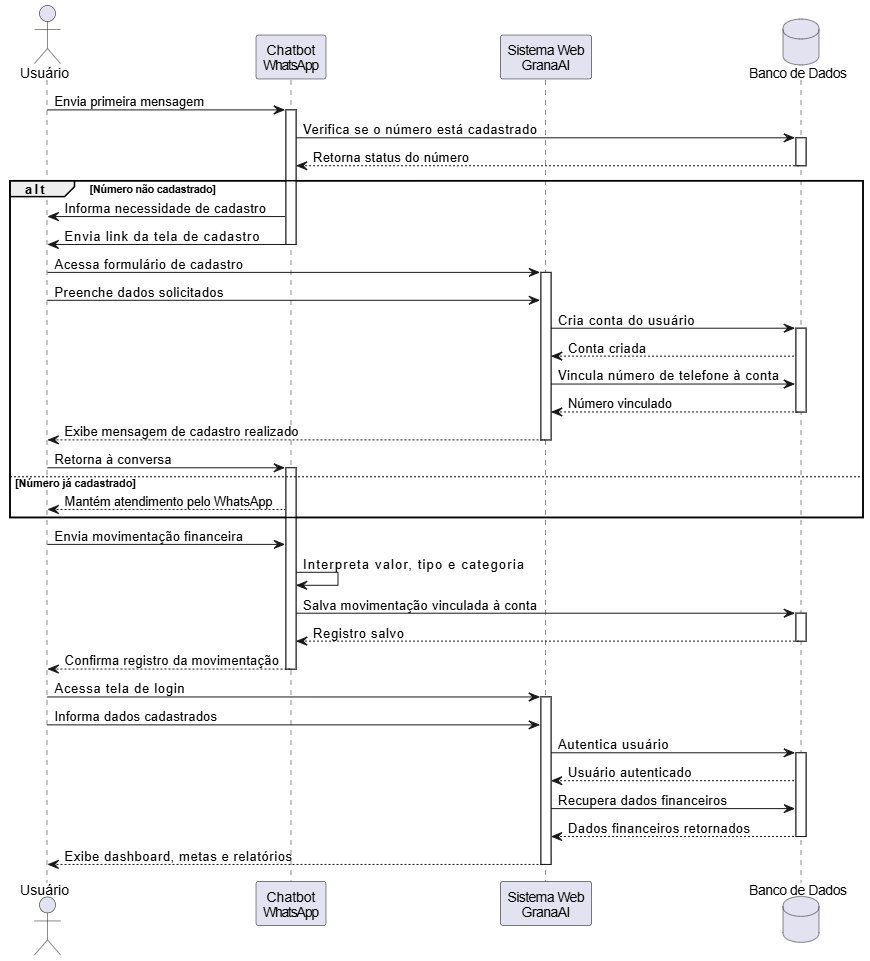
\includegraphics[width=\textwidth]{figs/diagrama-sequencia.png}
    \fonte{Elaborado pelos autores.}
\end{figure}

\subsubsection{Interface Conversacional (WhatsApp)}

A interação no WhatsApp foi projetada para ser rápida e intuitiva. O usuário pode enviar mensagens de texto ou áudio descrevendo um gasto, e o assistente GranaAI processa a informação em tempo real. A Figura \ref{fig:prototipo-whatsapp} ilustra uma simulação de uso onde o usuário registra uma compra impulsiva no iFood. Além de confirmar o registro, a IA fornece um \textit{insight} imediato sobre o limite da categoria, cumprindo o papel de assistente preventivo.

\begin{figure}[H]
    \centering
    \caption{Simulação de registro de gasto via WhatsApp}
    \label{fig:prototipo-whatsapp}
    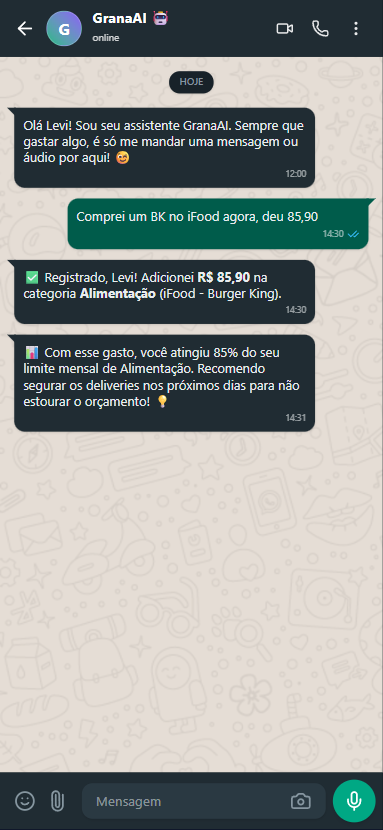
\includegraphics[width=0.5\textwidth]{figs/simulado-whatsapp.png}
    \fonte{Elaborado pelos autores.}
\end{figure}

\subsubsection{Dashboard Web}

A interface web serve como o centro de análise financeira do usuário. Nela, os dados registrados via WhatsApp são consolidados em visualizações gráficas que facilitam a compreensão do orçamento. A Figura \ref{fig:prototipo-dashboard} apresenta a visão geral do dashboard, com cartões de resumo financeiro, gráficos de evolução mensal e a lista de transações recentes.

\begin{figure}[H]
    \centering
    \caption{Interface principal do Dashboard Web}
    \label{fig:prototipo-dashboard}
    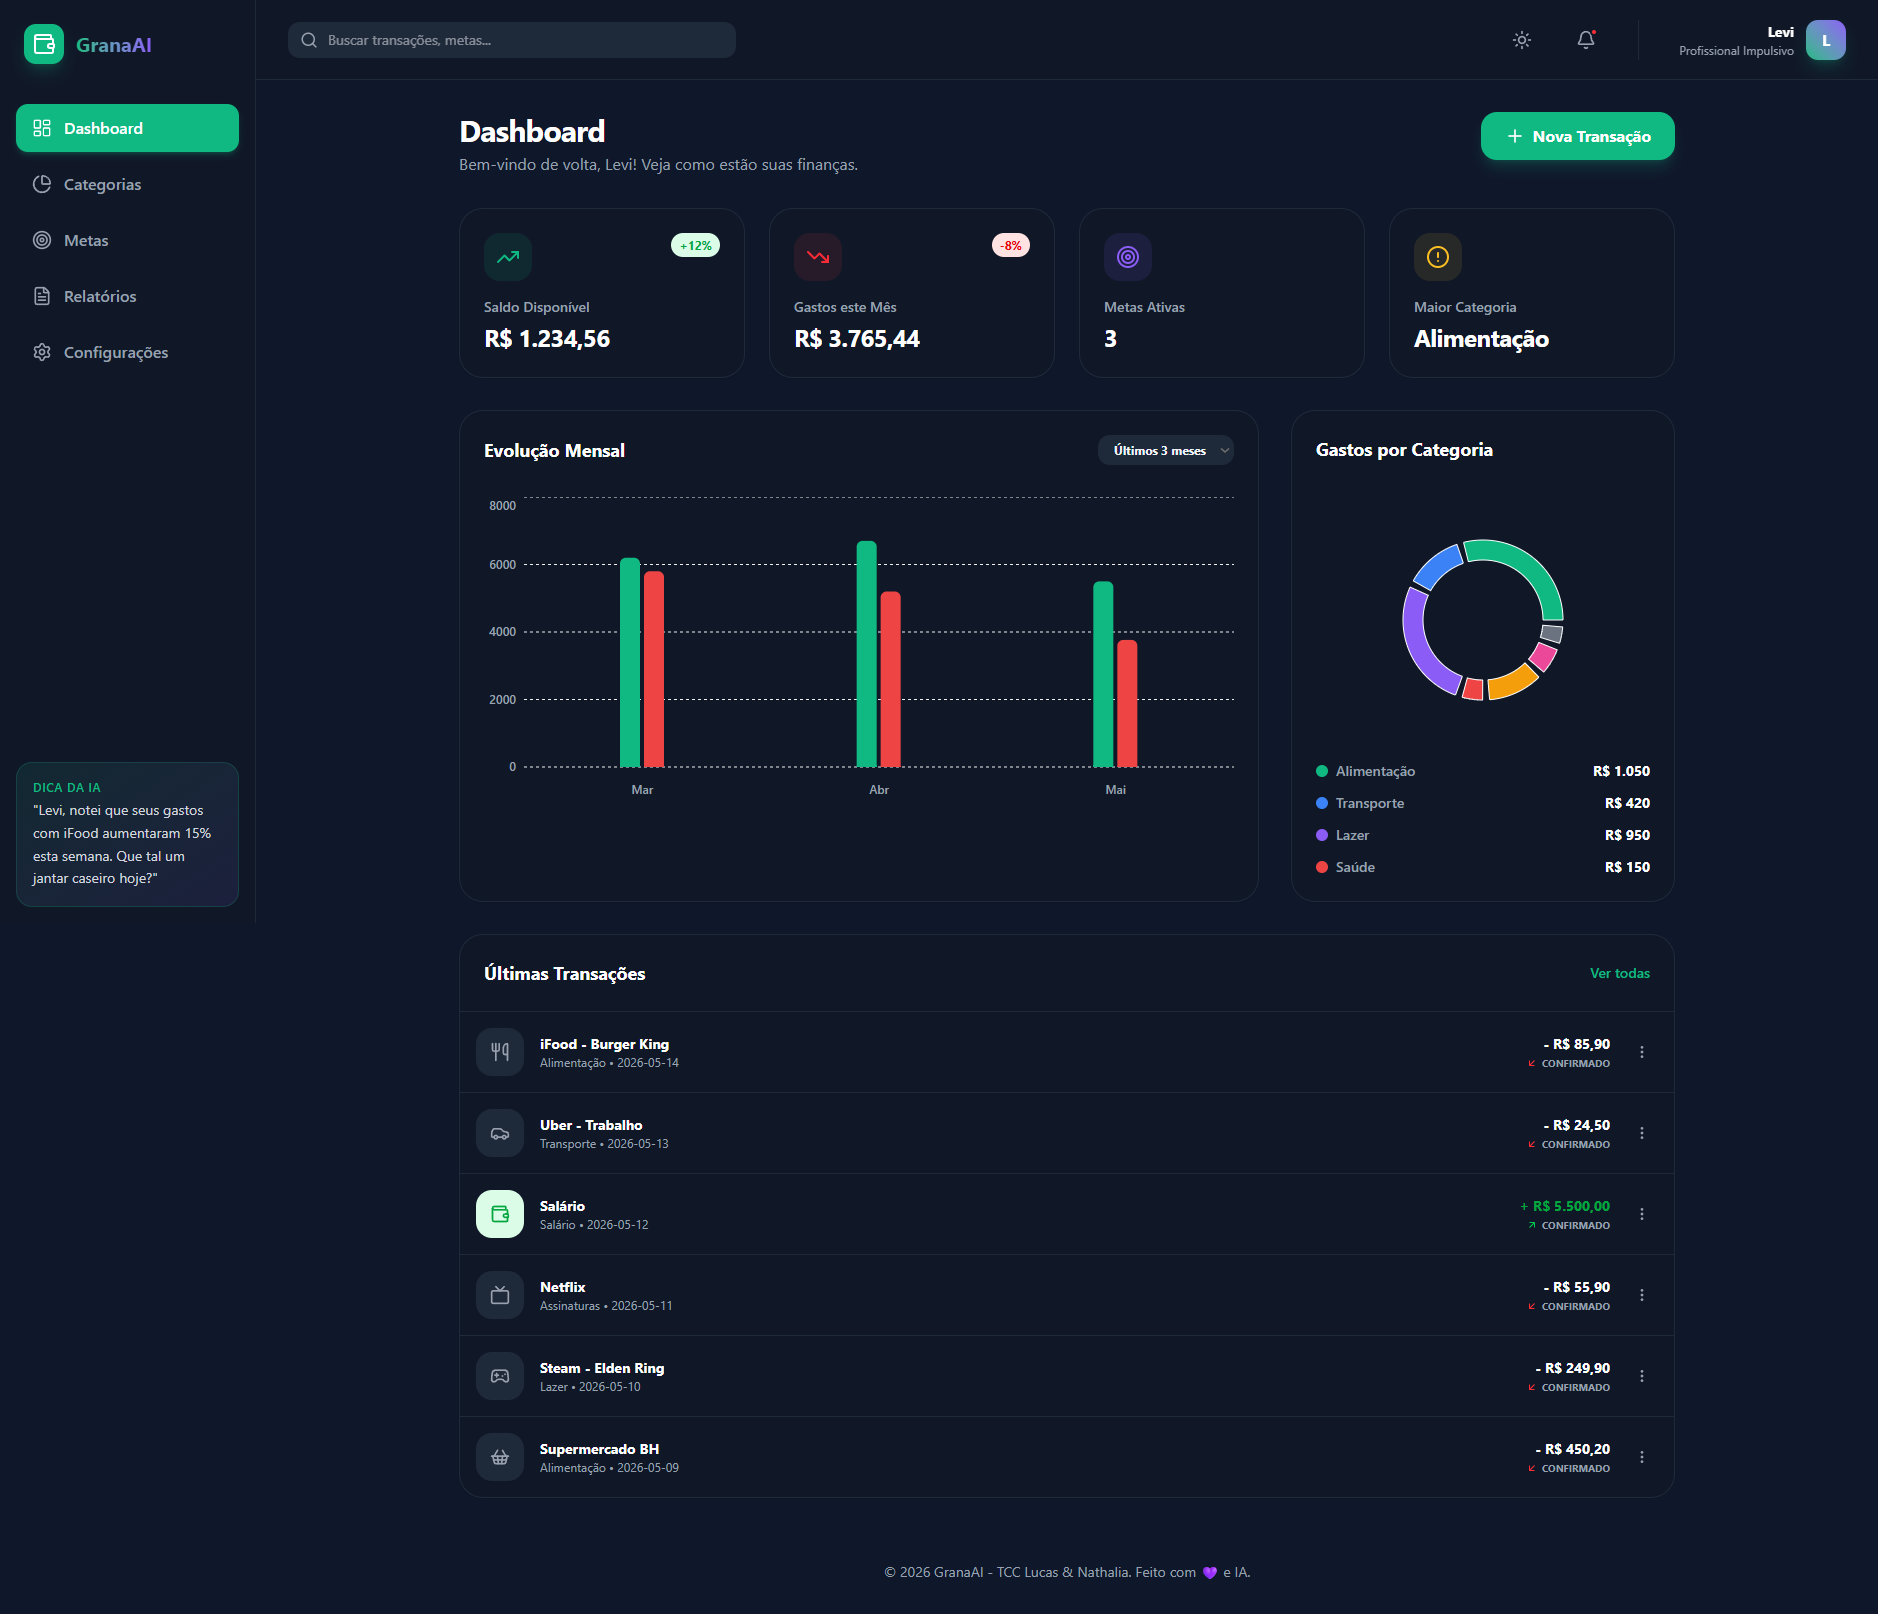
\includegraphics[width=\textwidth]{figs/dashboards.png}
    \fonte{Elaborado pelos autores.}
\end{figure}

As demais funcionalidades, como o gerenciamento de categorias (Figura \ref{fig:prototipo-categorias}) e o acompanhamento de metas financeiras (Figura \ref{fig:prototipo-metas}), complementam a experiência, permitindo que o usuário tenha controle total sobre seus objetivos de médio e longo prazo.

\begin{figure}[H]
    \centering
    \caption{Gerenciamento de limites por categoria}
    \label{fig:prototipo-categorias}
    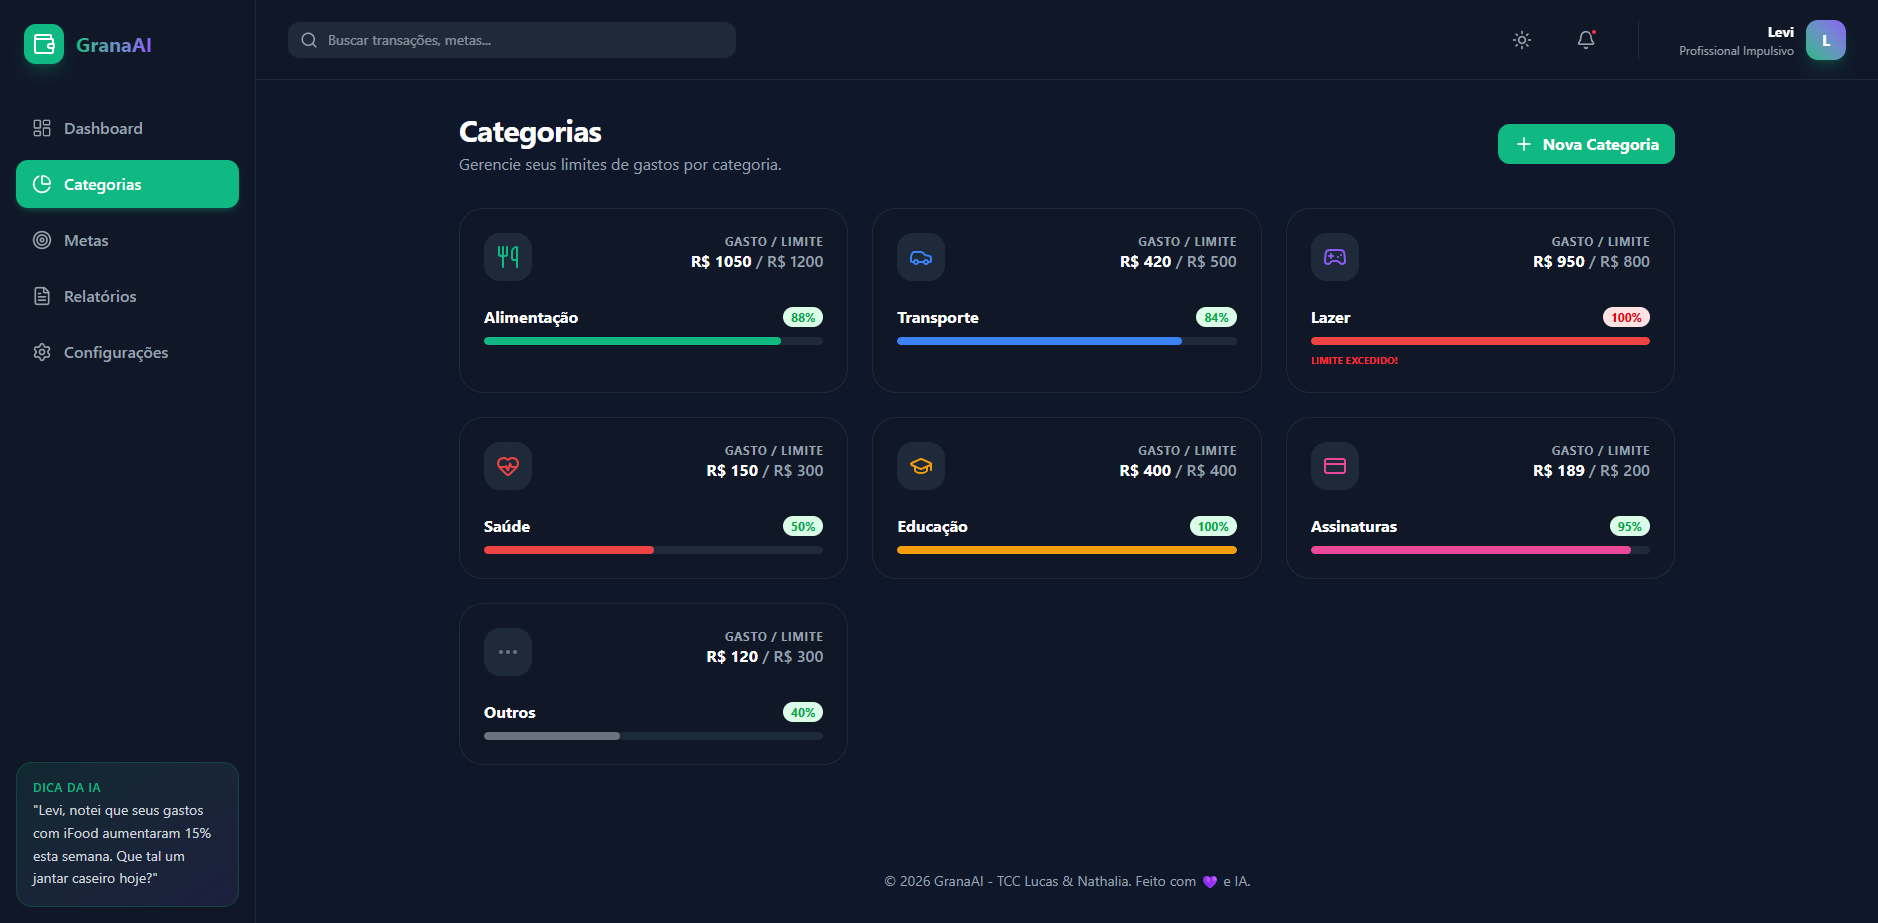
\includegraphics[width=0.8\textwidth]{figs/categorias.png}
    \fonte{Elaborado pelos autores.}
\end{figure}

\begin{figure}[H]
    \centering
    \caption{Acompanhamento de metas financeiras}
    \label{fig:prototipo-metas}
    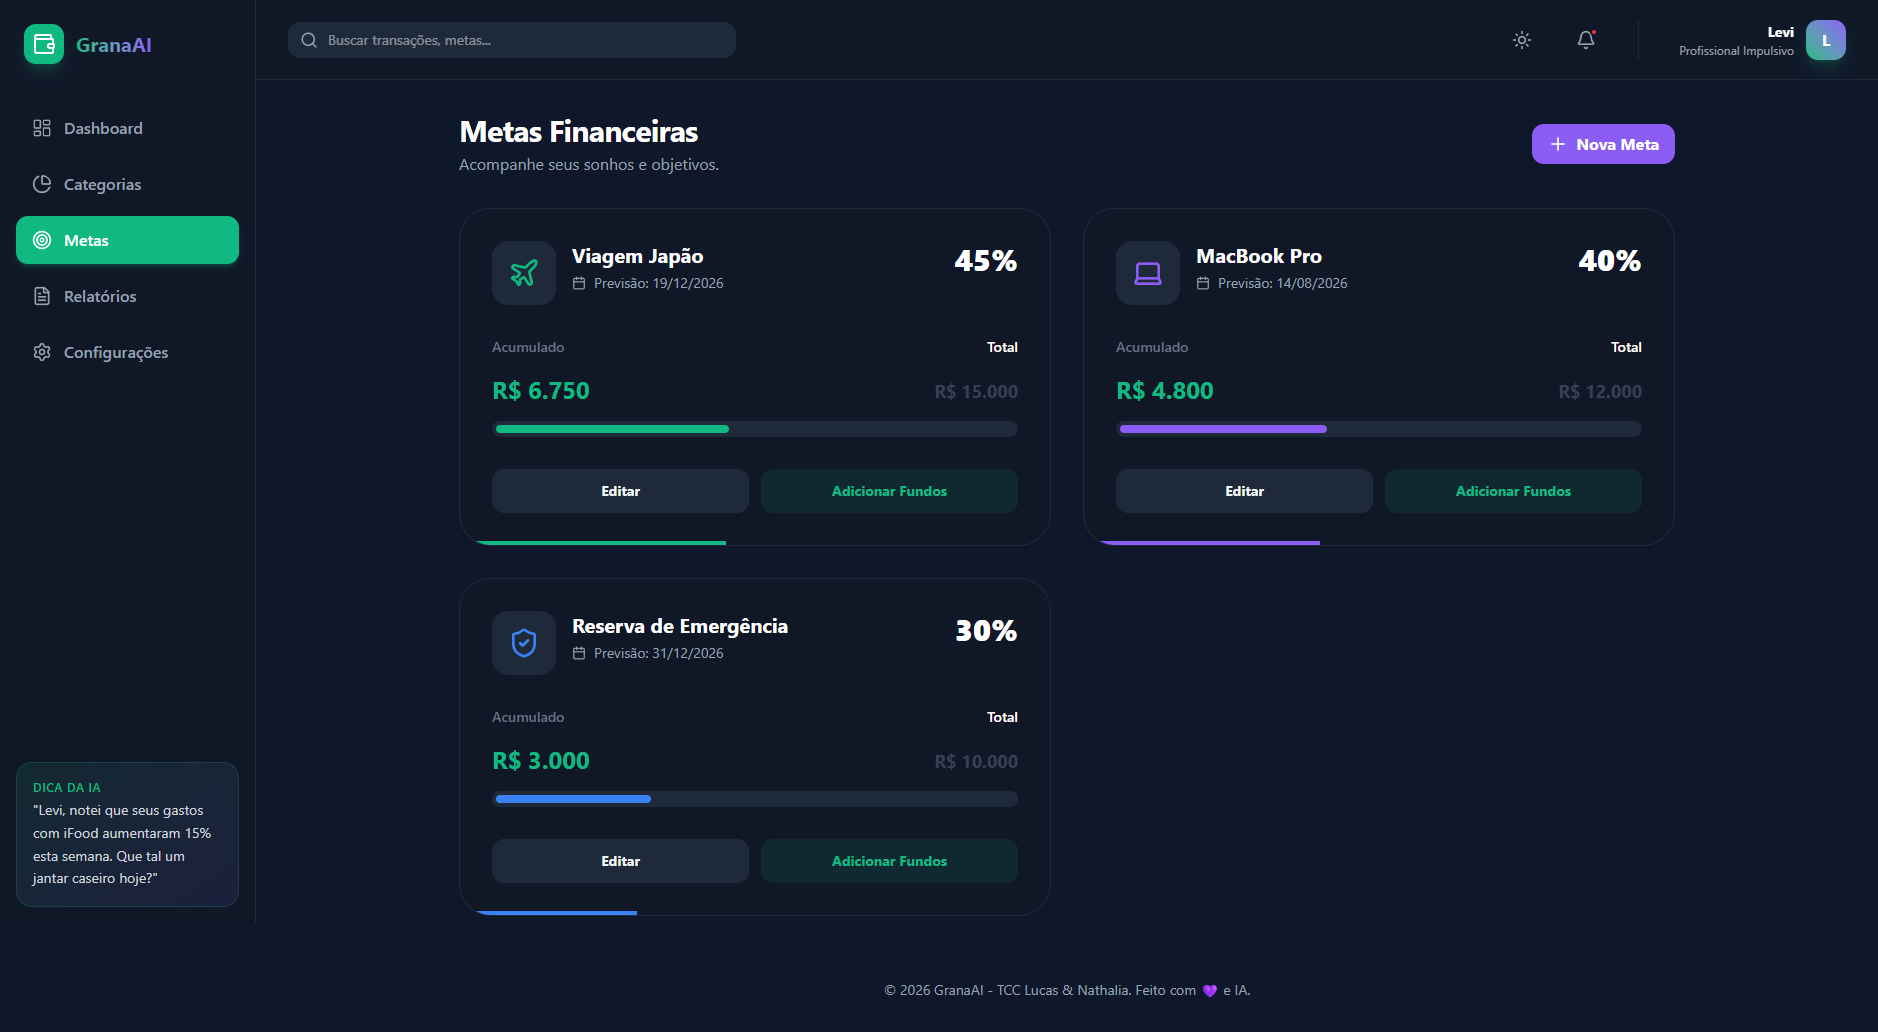
\includegraphics[width=0.8\textwidth]{figs/metas.png}
    \fonte{Elaborado pelos autores.}
\end{figure}

Por fim, a tela de relatórios e \textit{insights} (Figura \ref{fig:prototipo-relatorios}) oferece uma visão analítica e projeções futuras geradas pela IA, auxiliando na tomada de decisão estratégica do usuário.

\begin{figure}[H]
    \centering
    \caption{Relatórios detalhados e insights da IA}
    \label{fig:prototipo-relatorios}
    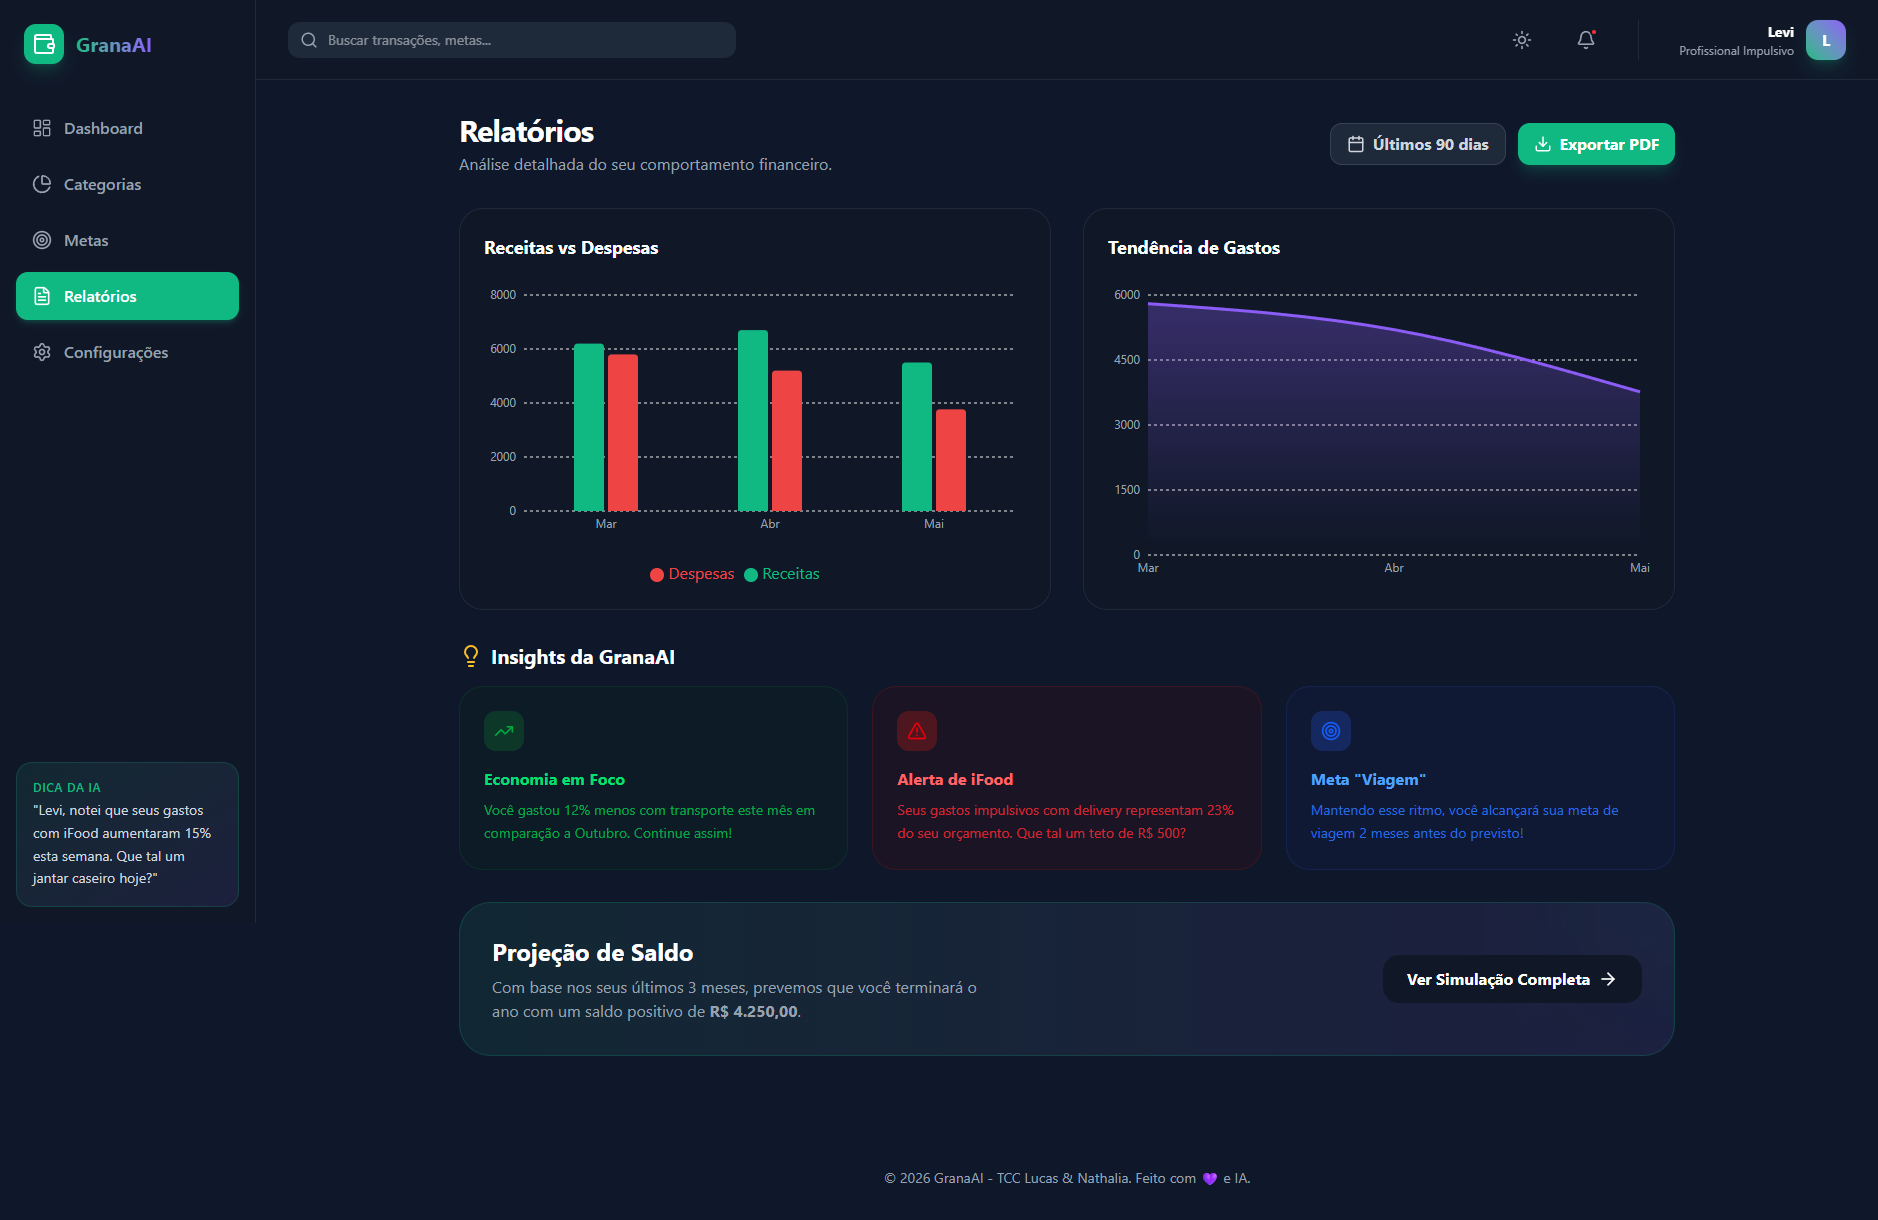
\includegraphics[width=\textwidth]{figs/relatorios.png}
    \fonte{Elaborado pelos autores.}
\end{figure}

\chapter{Conclusão}
Este trabalho teve como objetivo desenvolver uma abordagem automatizada para a resolução de jogos de adivinhação de palavras em português, utilizando técnicas de processamento de linguagem natural. A partir do desenvolvimento, implementação e experimentação da solução proposta, é possível afirmar que todos os objetivos específicos estabelecidos foram plenamente alcançados.

% A revisão dos trabalhos relacionados evidenciou que há múltiplas abordagens propícias para este tipo de problema, enfatizando o potencial dos modelos de aprendizado de máquina na captura de relações semânticas entre termos. Com base nesse embasamento teórico, foram selecionados três modelos amplamente utilizados — Word2Vec, GloVe e FastText —, todos treinados em corpus da língua portuguesa, a fim de avaliar o desempenho de cada um no desafio proposto.

% Os resultados obtidos demonstraram que o sistema desenvolvido, implementado em Python e integrado ao jogo por meio do Playwright, foi capaz de encontrar a palavra secreta em uma proporção significativa das execuções realizadas, comprovando a eficácia da abordagem. Entre os modelos avaliados, o GloVe apresentou o melhor desempenho, destacando-se por alcançar a maior taxa de acertos.

% Portanto, constata-se que a utilização de embeddings semânticos para automatizar a resolução de jogos linguísticos não é apenas viável, mas também eficaz, reforçando o potencial dessas técnicas em aplicações voltadas ao entretenimento, à educação e ao aprimoramento de modelos de linguagem em português.

Foi desenvolvido um sistema completo para a resolução automática de partidas do jogo Contexto, incluindo a estruturação da classe ContextoSolver, a integração com o Playwright e a criação de módulos auxiliares. Em seguida, uma heurística de seleção de palavras foi implementada, combinando similaridade semântica, exploração inicial e um modo de otimização com Regressão Ridge, abordagem responsável por guiar o processo de busca e aprimorar dinamicamente as escolhas do algoritmo durante a partida.

Quanto à avaliação da eficiência dessa heurística, foram conduzidos experimentos em mil execuções, registrando taxa de acertos e quantidade de tentativas. Os resultados demonstraram que a heurística é funcional, consistente e capaz de resolver uma parcela significativa das partidas.

Além disso, foi realizada uma investigação estruturada de diferentes modelos de word embeddings incluindo o estudo de suas características e sua aplicação prática na resolução automática. Tal exploração permitiu compreender suas diferenças, capacidades e limitações no contexto do projeto. O sistema desenvolvido foi capaz de comparar o desempenho desses modelos sob a mesma heurística, garantindo uma análise justa e padronizada.

Com isso, o projeto cumpriu seus objetivos específicos, tais como a criação de um sistema funcional de automação, o desenvolvimento de uma heurística eficaz de seleção de palavras, a avaliação de sua eficiência por meio de experimentos sistemáticos e a comparação estruturada entre diferentes modelos de word embeddings, destacando o GloVe como o mais adequado à tarefa.

\section{Trabalhos Futuros}

Como desdobramento deste estudo, é possível diversas oportunidades de aprimoramento e expansão da solução proposta. Uma primeira vertente consiste na otimização da estratégia de seleção de palavras através de algoritmos de Aprendizado por Reforço, como o Q-Learning. Conforme explorado na revisão bibliográfica, essa abordagem permitiria que o agente aprendesse uma política de escolha ótima baseada nas recompensas (ranking) recebidas a cada tentativa, visando reduzir o número total de interações necessárias para encontrar a palavra secreta.

Outra possibilidade relevante é a implementação de uma estratégia de heurística híbrida ou dinâmica. Um trabalho futuro poderia investigar o uso de um modelo com maior capacidade de generalização para a etapa de exploração inicial, alternando automaticamente para um modelo com maior precisão local ou ajustado para sinônimos na etapa de refinamento, quando o ranking se aproxima do alvo. Adicionalmente, técnicas de Ensemble, que combinam a votação de múltiplos modelos para decidir a próxima jogada, poderiam mitigar as fraquezas individuais de cada arquitetura.

Recomenda-se também a investigação de abordagens baseadas em \textit{Graph Embeddings} e grafos de conhecimento. Diferente dos modelos vetoriais tradicionais, que dependem puramente de distâncias cosseno em um espaço denso, modelar o vocabulário como um grafo, onde os vértices são palavras e as arestas representam o peso da proximidade semântica, permitiria explorar algoritmos de caminho mínimo ou detecção de comunidades. Isso poderia solucionar casos onde a similaridade vetorial falha em capturar relações diretas, como hiperônimos ou termos técnicos específicos.

Por fim, propõe-se a evolução da ferramenta para suportar um formato de torneio de agentes autônomos, inspirado na dinâmica de competições de robótica. Nessa estrutura, o sistema desenvolvido atuaria como uma "arena" padronizada, aproveitando sua arquitetura modular. Pesquisadores e estudantes seriam desafiados a submeter seus próprios "robôs de software", compostos por modelos treinados em corpora personalizados e heurísticas ajustadas, para competir na resolução simultânea de desafios. Essa abordagem fomentaria a busca prática por eficiência, premiando soluções que demonstrem maior criatividade na engenharia de dados e na otimização algorítmica.
\clearpage
\thispagestyle{empty}

Durante a preparação deste trabalho, o(a) autor(a) utilizou Gemini e ChatGPT para revisão gramatical, sugestão de paráfrase, apoio na organização textual e apoio na estruturação do protótipo.

Após utilizar a ferramenta, o(a) autor(a) revisou e editou o conteúdo conforme necessário, e assume total responsabilidade pelo conteúdo da publicação.

\clearpage

% \input{cap6}

% ----------------------------------------------------------
% Finaliza a parte no bookmark do PDF
% para que se inicie o bookmark na raiz
% e adiciona espaço de parte no Sumário
% ----------------------------------------------------------
\phantompart

% ---
% Conclusão
% ---
%\chapter{Conclusão}
% ---

% ----------------------------------------------------------
% ELEMENTOS PÓS-TEXTUAIS
% ----------------------------------------------------------
\postextual
% ----------------------------------------------------------

% ----------------------------------------------------------
% Referências bibliográficas estilo min
% ----------------------------------------------------------
\citeoption{abnt-etal-list=5}
\bibliographystyle{abntex2-cite-min}


\bibliography{TCC.bib}

% ----------------------------------------------------------
% Glossário
% ----------------------------------------------------------
%
% Consulte o manual da classe abntex2 para orientações sobre o glossário.
%
%\glossary

%\include{apendices}

%\include{anexos}

%---------------------------------------------------------------------
% INDICE REMISSIVO
%---------------------------------------------------------------------
\phantompart
\printindex
%---------------------------------------------------------------------

\end{document}
